\documentclass[11pt, notitlepage]{report}

\usepackage{amssymb}
\usepackage{amsmath}
\usepackage{multicol}
\usepackage{graphicx}
\usepackage{epigraph}
\usepackage{chngpage}
\usepackage{fancyhdr}
\usepackage[braket, qm]{qcircuit}
\usepackage[font={small, it}, labelfont=bf, skip=3pt]{caption}
\usepackage[hidelinks]{hyperref}
\usepackage{subcaption}
\usepackage[normalem]{ulem}
\usepackage{tikz}
\usepackage{sectsty}
\usepackage{etoolbox}
\usepackage{titlesec}
\usepackage{dirtytalk}
\usepackage{times}
\usepackage{pgfplots}

\titleformat{\chapter}[display]   
{\normalfont\LARGE\bfseries}{\chaptertitlename\ \thechapter}{20pt}{\huge}   
\titlespacing*{\chapter}{0pt}{-50pt}{15pt}

\usepgflibrary{arrows}

%% Gate matrices and quantum state vectors
\newcommand{\igate}{
  \begin{pmatrix}
  1 & 0 \\
  0 & 1
  \end{pmatrix}
}
\newcommand{\xgate}{
  \begin{pmatrix}
  0 & 1 \\
  1 & 0
  \end{pmatrix}
}
\newcommand{\ygate}{
  \begin{pmatrix}
  0 & -i \\
  i & \phantom{-}0
  \end{pmatrix}
}
\newcommand{\zgate}{
  \begin{pmatrix}
  1 & \phantom{-}0 \\
  0 & -1
  \end{pmatrix}
}
\newcommand{\hgate}{
  \dfrac{1}{\sqrt2}
  \begin{pmatrix}
  1 & \phantom{-}1 \\
  1 & -1
  \end{pmatrix}
}
\newcommand{\sgate}{
  \begin{pmatrix}
  1 & 0 \\
  0 & i
  \end{pmatrix}
}
\newcommand{\phasegate}{
  \begin{pmatrix}
  1 & \phantom{e}0 \\
  0 & e^{i\theta}
  \end{pmatrix}
}
\newcommand{\cnotgate}{
  \begin{pmatrix}
  1 & 0 & 0 & 0 \\
  0 & 1 & 0 & 0 \\
  0 & 0 & 0 & 1 \\
  0 & 0 & 1 & 0 \\
  \end{pmatrix}
}

\newcommand{\qstatezero}{
  \begin{pmatrix}1 \\ 0\end{pmatrix}
}
\newcommand{\qstateone}{
  \begin{pmatrix}0 \\ 1\end{pmatrix}
}

\setlength\epigraphwidth{10cm}
\setlength\epigraphrule{0pt}

\makeatletter
\patchcmd{\epigraph}{\@epitext{#1}}{\itshape\@epitext{#1}}{}{}
\newcommand*{\toccontents}{\@starttoc{toc}}
\makeatother

\renewcommand*{\arraystretch}{1.1}

\pagestyle{fancy}
\lhead{}

\title{\textbf{Introduction to Quantum Computing \\
\large Lectures by Leon Riesebos}}
\author{Steven Oud \\ \emph{soud@pm.me}}
\begin{document}
     
\maketitle

\toccontents

\newpage

\chapter{Fundamentals: A One-Qubit World}
\epigraph{Quantum computers are machines that rely on characteristically quantum phenomena, such as quantum interference and quantum entanglement, in order to perform computation.}{--- Artur Ekert}

\epigraph{It is tempting to say that a quantum computer is one whose operation is governed by the laws of quantum mechanics. But since the laws of quantum mechanics govern the behavior of all physical phenomena, this temptation must be resisted. Your laptop operates under the laws of quantum mechanics, but it is not a quantum computer.}{--- N. David Mermin}

\section{The Qubit}
A quantum bit (\emph{qubit}) - like a classical bit - has a \emph{state}. In classical bits this is 0 or 1. Two possible states for a qubit are \ket{0} and \ket{1} (denoted in \emph{Dirac notation}), which correspond to the states 0 and 1 for a classical bit. The difference between bits and qubits is that a qubit can be in other states than \ket{0} or \ket{1}, called \emph{superpositions}. The state of a qubit can be denoted as following:
\begin{equation}
  \ket{\psi} = \alpha\ket{0} + \beta\ket{1},
\end{equation}
where $\alpha$ and $\beta$ are complex numbers. The special states \ket{0} and \ket{1} are known as \emph{computational basis states}. We cannot examine a qubit to determine its quantum state. Quantum mechanics tells us we can only acquire much more restricted information about the quantum state. When we measure a qubit we get either 0, with probability $|\alpha|^2$, or 1, with probability $|\beta|^2$. The sum of all probabilities is always equal to 1:
\begin{equation}
  |\alpha|^2 + |\beta|^2 = 1.
\end{equation}
For example, a qubit in the state
\begin{equation}
  \dfrac{1}{\sqrt2}\ket{0}+\dfrac{1}{\sqrt2}\ket{1}
\end{equation}
gives 0 fifty percent of the time ($|1/\sqrt2|^2$), and 1 fifty percent of the time. This state is often denoted by \ket{+}.

\section{The Bloch Sphere}
The Bloch sphere is a geometrical representation of a qubit's state. It's a spherical coordinate system in which a quantum state can be described as
\begin{equation}
  \ket{\psi} = e^{i\delta} \left(\cos\dfrac{\theta}{2}\ket{0} + e^{i\phi}\sin\dfrac{\theta}{2}\ket{1}\right),
\end{equation}
where $\delta, \theta$ and $\phi$ are real numbers. Factor $e^{i\delta}$ is the global phase of the state. This factor does not influence measurement probabilities, since $\left|e^{i\delta}\right| = 1$. Therefore we can often omit it, allowing us to write
\begin{equation}
  \ket{\psi} = \cos\dfrac{\theta}{2}\ket{0} + e^{i\phi}\sin\dfrac{\theta}{2}\ket{1}.
\end{equation}
The numbers $\theta$ and $\phi$ define a point on the three-dimensional sphere (Figure~\ref{fig:bloch}). The Bloch sphere visualization can be very useful for describing single qubit operations. It is however limited in that there is no simple generalization of the Bloch sphere known for multiple qubits.
\begin{figure}[ht]
  \centering
  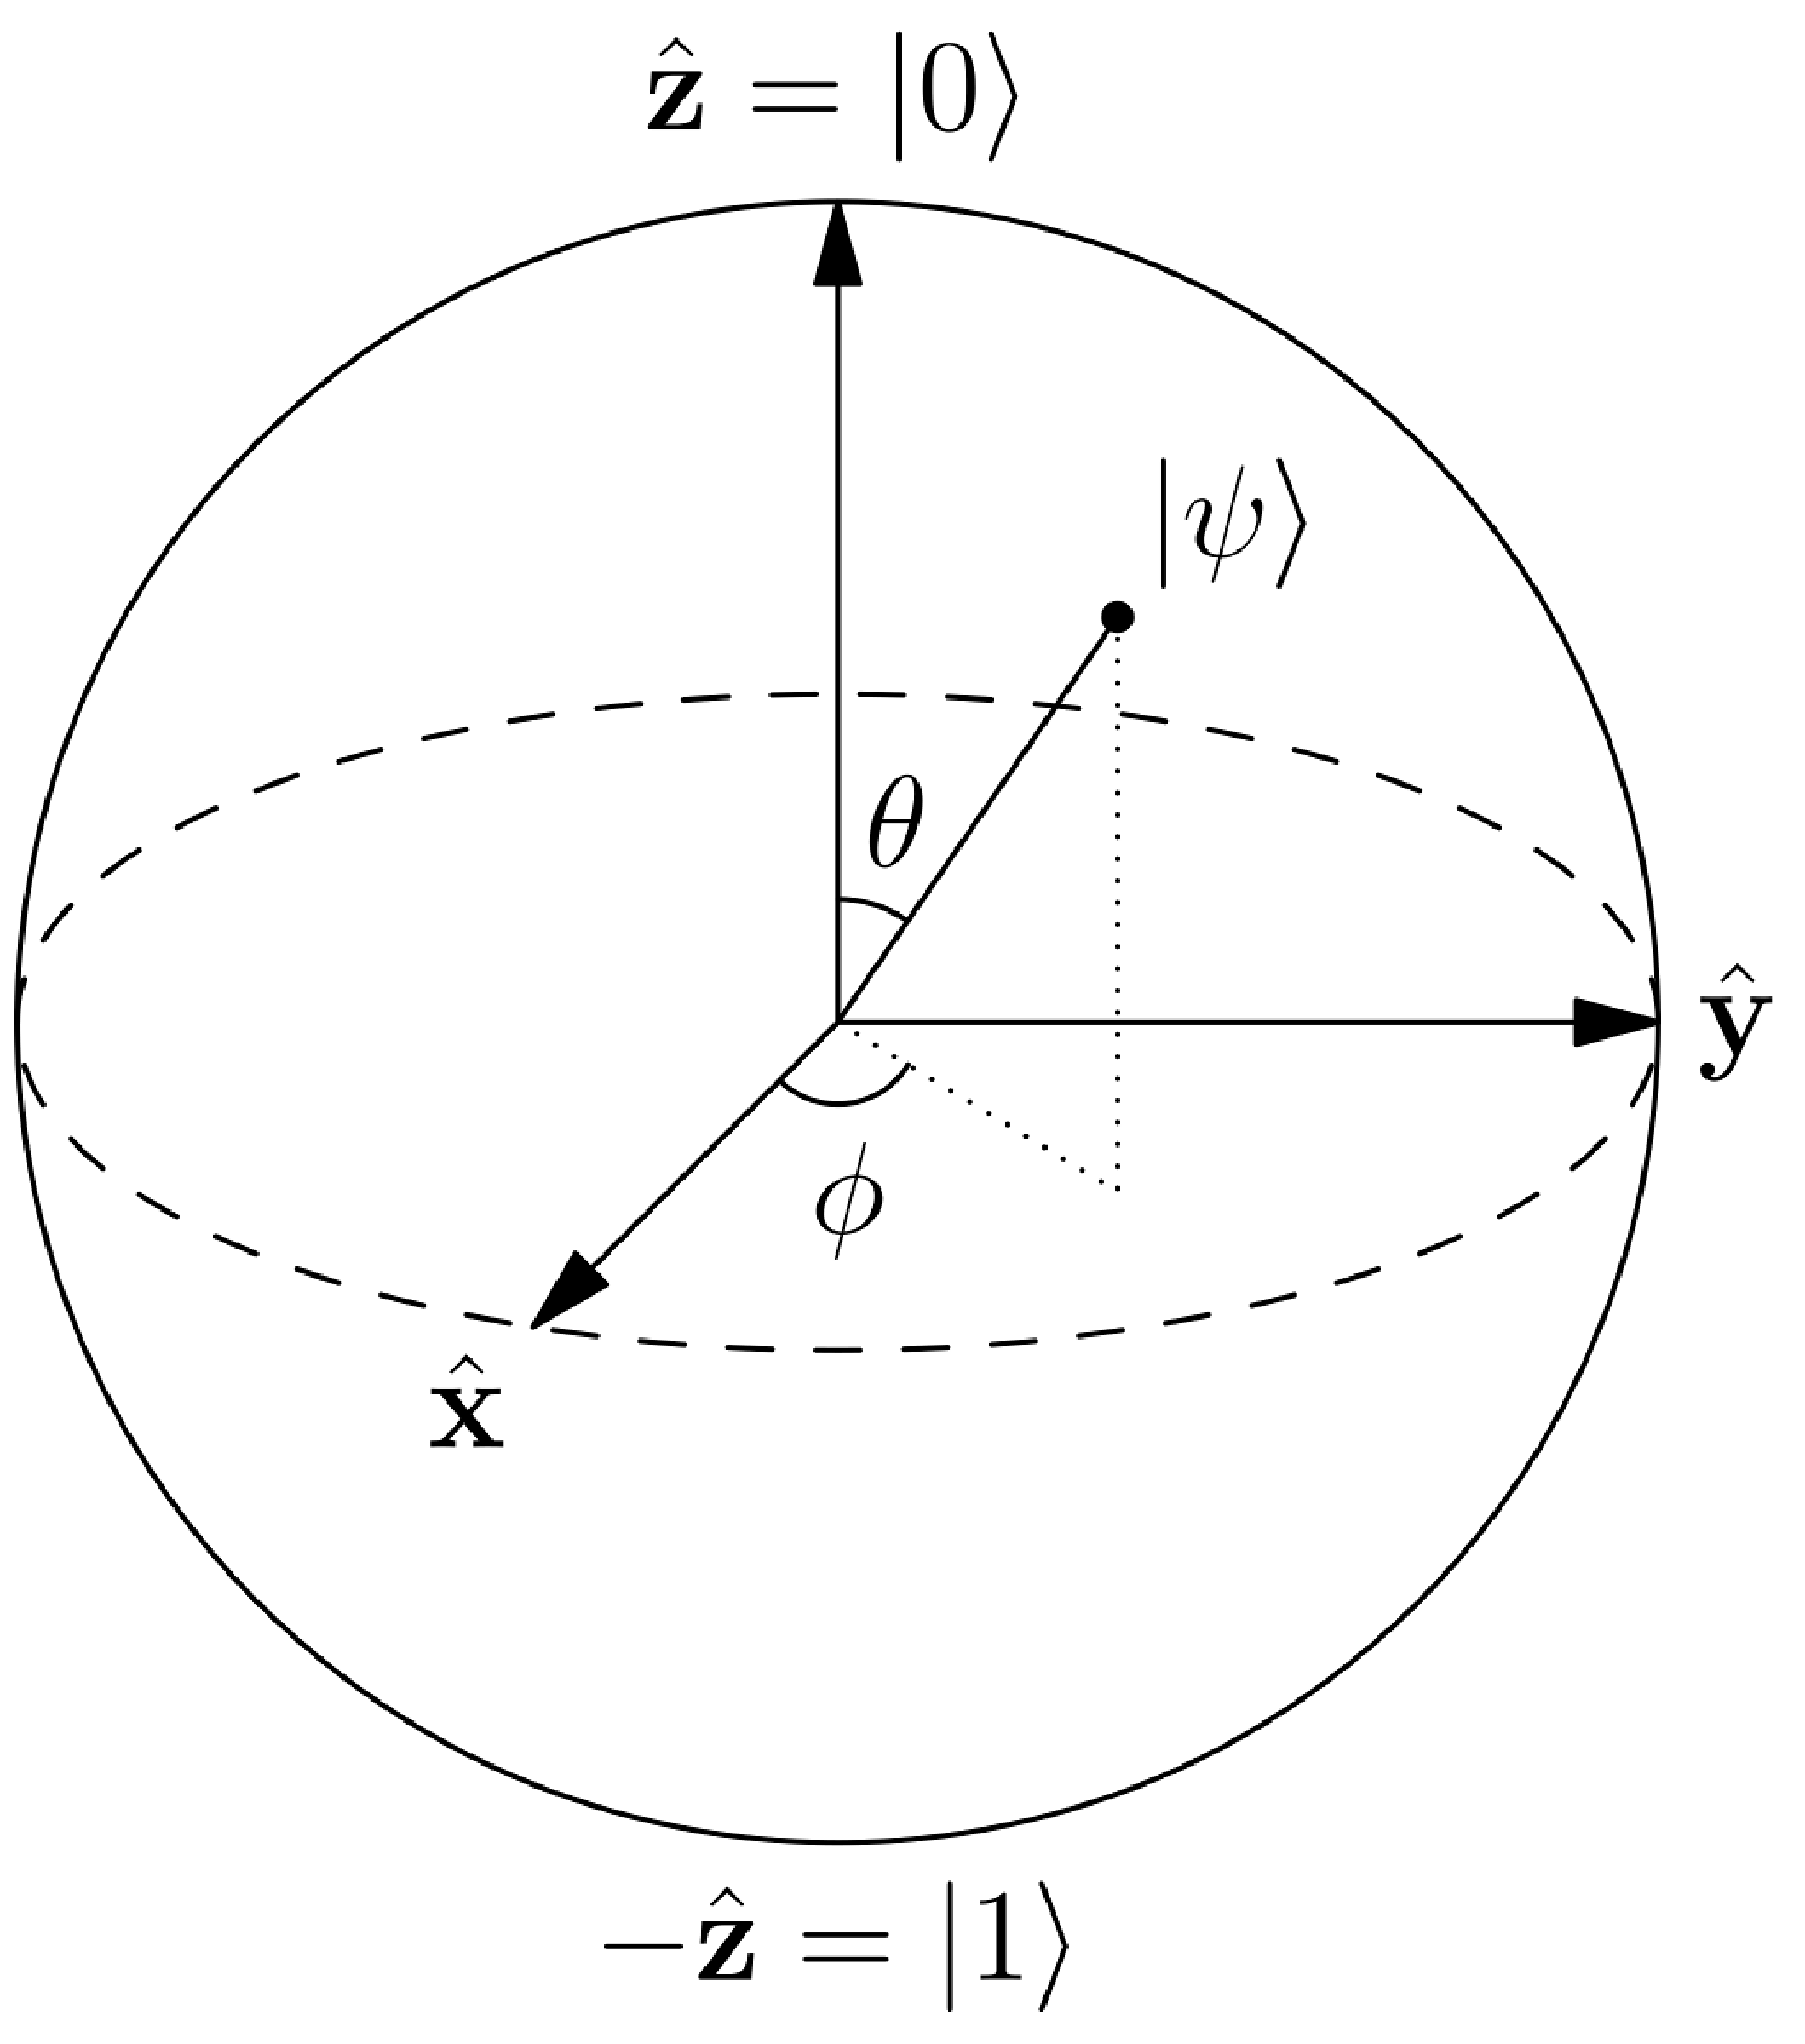
\includegraphics[scale=0.175]{images/bloch_sphere.eps}
  \vspace{2mm}
  \caption{Bloch sphere representation of a qubit.}
  \label{fig:bloch}
\end{figure}
\par
\newpage

\section{Single-Qubit Quantum Gates}
Single-qubit quantum gates can be seen as counter-clockwise rotations on the Bloch sphere. These gates only have one limitation: they have to be \emph{unitary}, that is $U^\dagger U = UU^\dagger = I$, where $U^\dagger$ is the conjugate transpose of $U$ and $I$ the identity operation. Therefore, any $2^n \times 2^n$ unitary operation is a valid gate which acts on $n$ qubits. We will often use circuit notation to describe the transformation of state \ket{\psi} to \ket{\psi'} by a unitary operation $U$ as following:
\[
  \Large{
  \Qcircuit @C=1em @R=0em {
    & \lstick{\ket{\psi}} & \gate{U} & \qw & \ket{\psi'}
  }
}
\]
Below are some notable single-qubit gates described and visualized.

\subsection{Pauli Gates}\label{pauli_gates}
 The most simple quantum gates are the \emph{Pauli gates} $I$, $X$, $Y$ and $Z$. $I$ is the identity gate, which does nothing. The other gates rotate $\pi$ radians (180 degrees) around the X, Y or Z-axis. These gates are self-inverse, meaning $U^2 = I$.

\begin{figure}[ht]
  \centering
  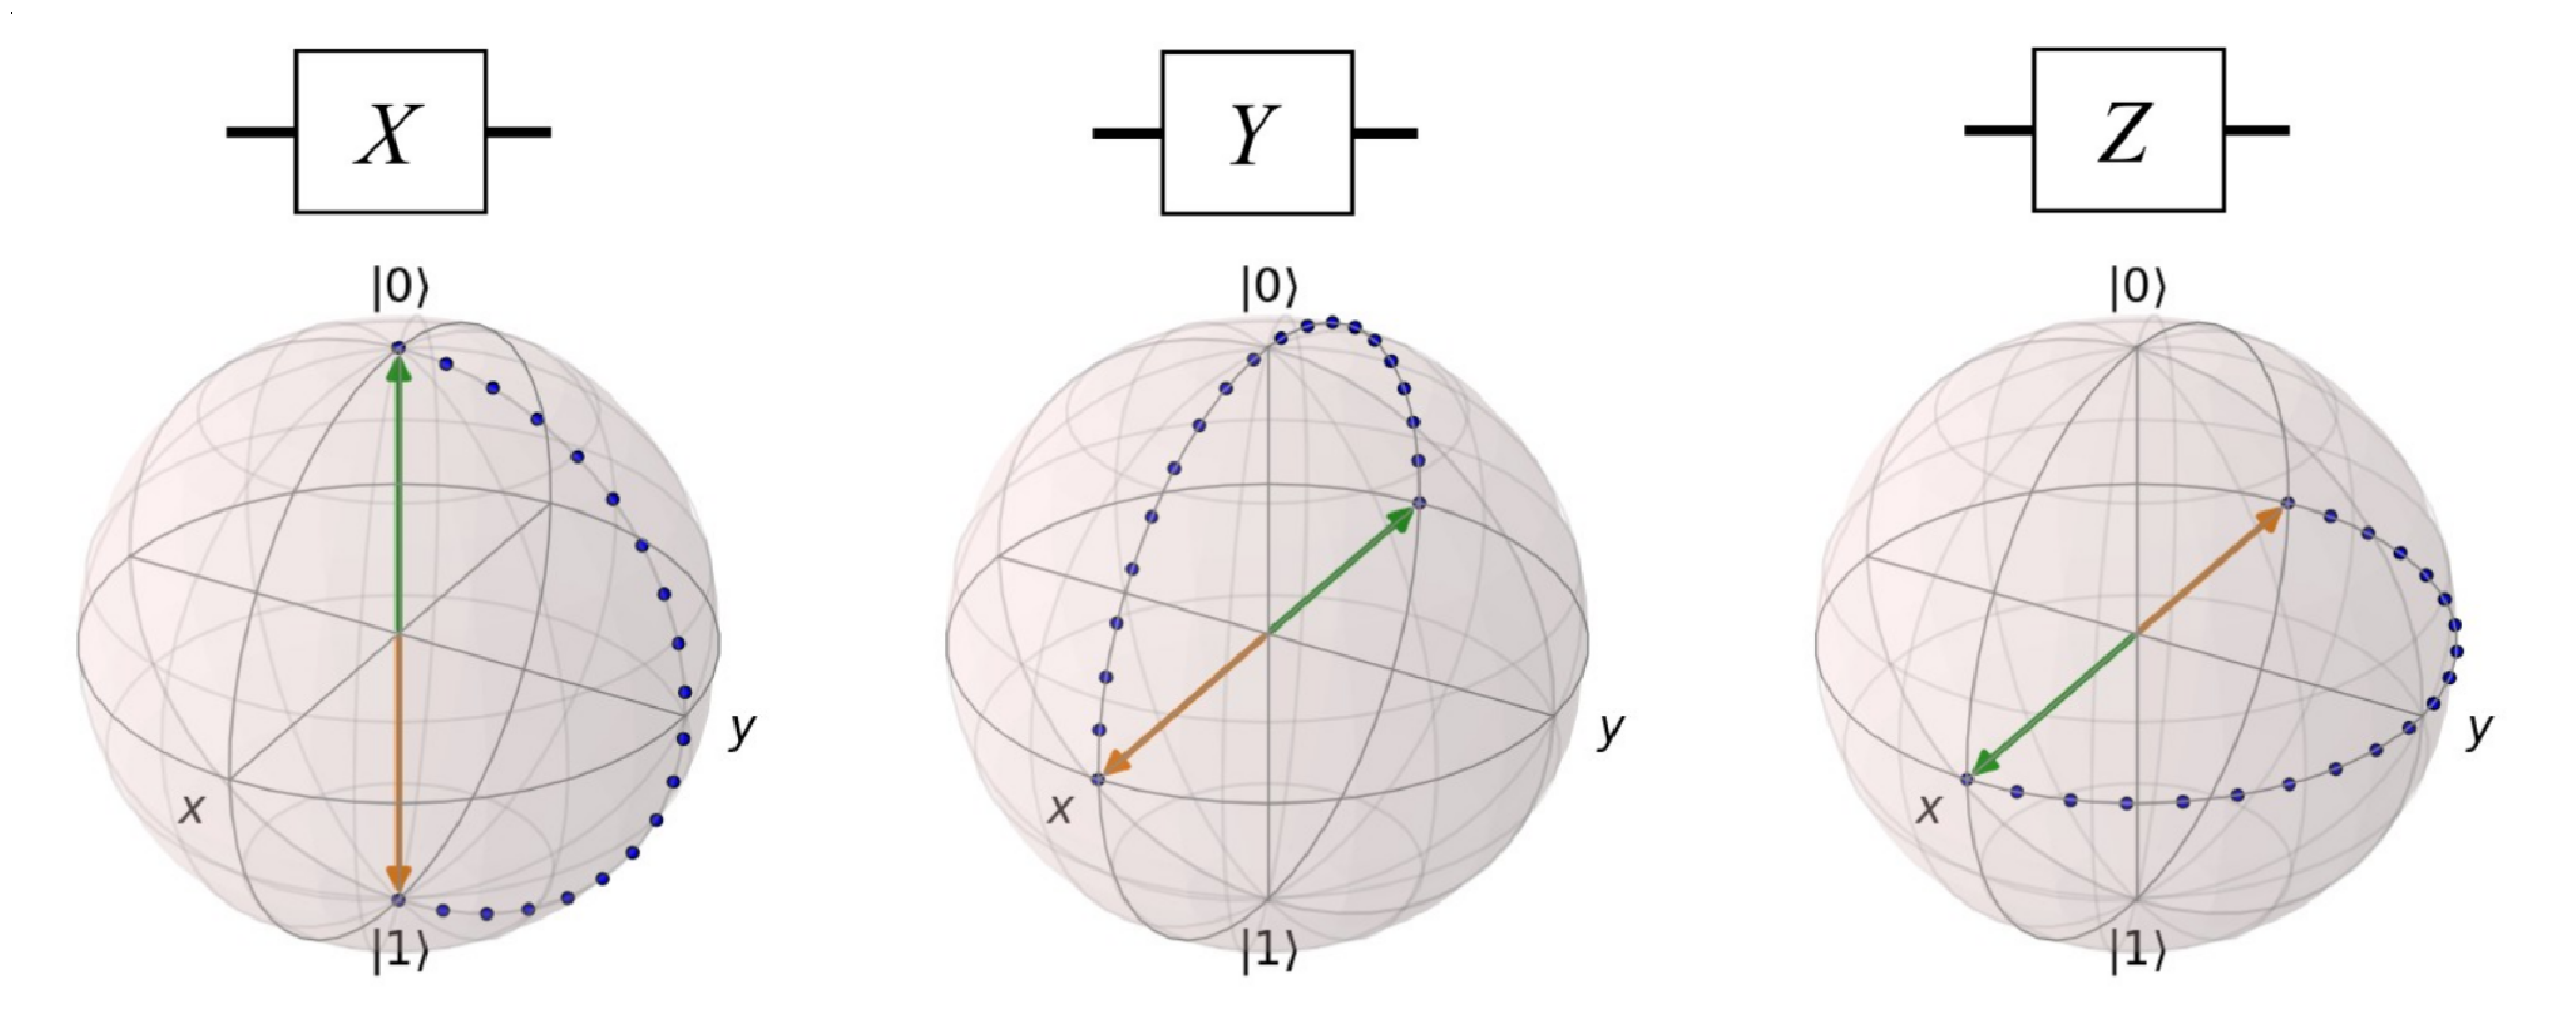
\includegraphics[scale=0.175]{images/pauli_gates.eps}
  \vspace{2mm}
  \caption{Pauli gates $X$, $Y$ and $Z$ visualized on the Bloch sphere. The green vector is the starting position and the orange vector the final position.}
\end{figure}

\subsection{Hadamard Gate}
The \emph{Hadamard} ($H$) gate maps the basis states \ket{0} and \ket{1} to superposition states with equal weight:
\begin{align}
H\ket{0} = \ket{+} &= \dfrac{1}{\sqrt2}(\ket{0} + \ket{1}) \\
H\ket{1} = \ket{-} &= \dfrac{1}{\sqrt2}(\ket{0} - \ket{1}).
\end{align}
It is the combination of two rotations, $\pi$ radians about the Z-axis followed by $\pi/2$ radians about the Y-axis. This gate is sometimes described as a ``square root of \textsc{not}" gate. The Hadamard gate belongs to the Clifford gates.

\begin{figure}[ht]
    \centering
    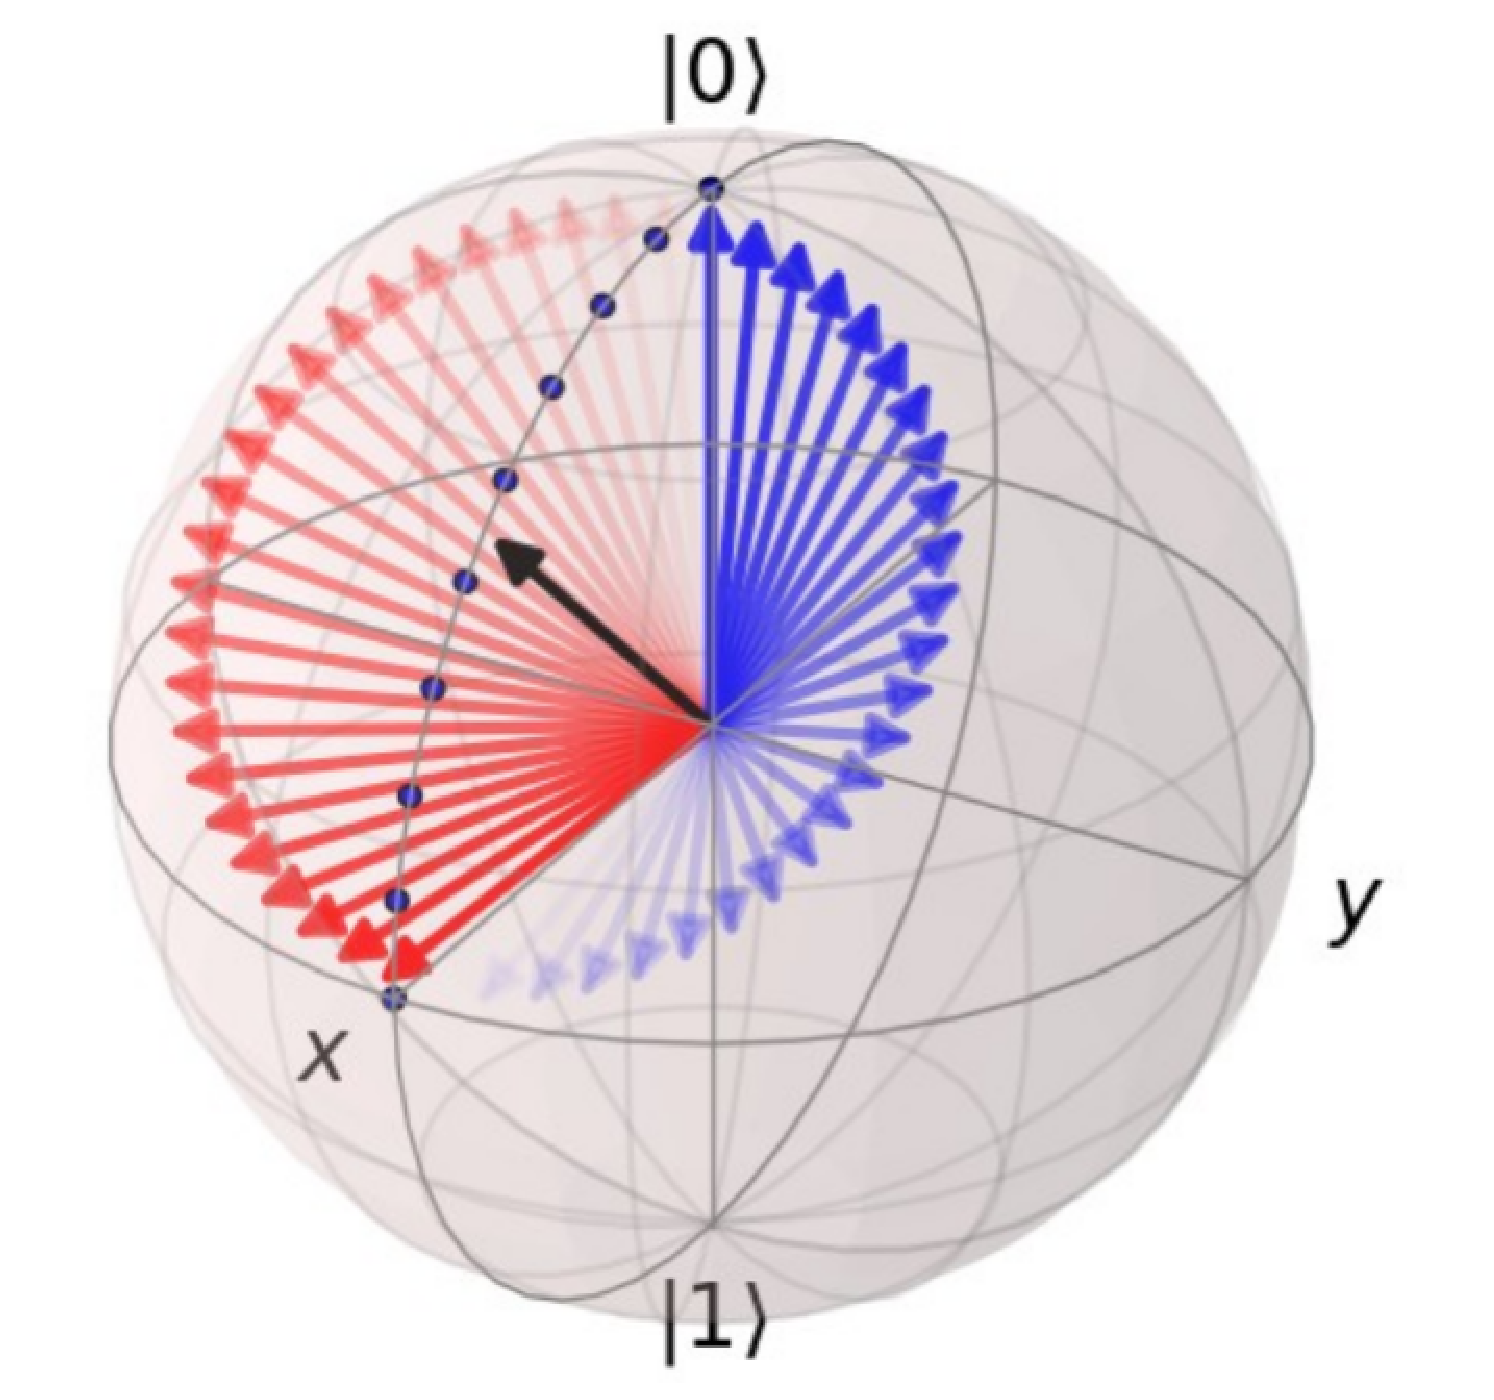
\includegraphics[scale=0.165]{images/hadamard_gate.eps}
    \vspace{1mm}
    \caption{Hadamard gate visualized on the Bloch sphere.}
\end{figure}

\subsection{Phase Gates}
Rotation gates that rotate around the Z axis are considered \emph{phase gates}. They rotate the phase of the \ket{1} state by an angle $\theta$ and leave the \ket{0} state unchanged:
\begin{equation}
\begin{aligned}
R_z(\theta) \ket{0} &= \ket{0} \\
R_z(\theta) \ket{1} &= e^{i\theta}\ket{1}.
\end{aligned}
\end{equation}
The probability of measuring a \ket{0} or \ket{1} is unchanged after a phase gate, however it modifies the phase of the quantum state. A common phase gate is the \emph{S gate}, where $\theta = \pi/2$ (Figure \ref{fig:s_bloch}). The Pauli Z gate can be thought of as a phase gate where $\theta = \pi$, because $e^{i\pi} = -1$. Thus you could also think of the $S$ gate as half a Pauli Z gate. Another common phase gate is the \emph{T gate}, where $\theta = \pi/4$ (half an $S$ gate).

\begin{figure}[ht]
  \centering
  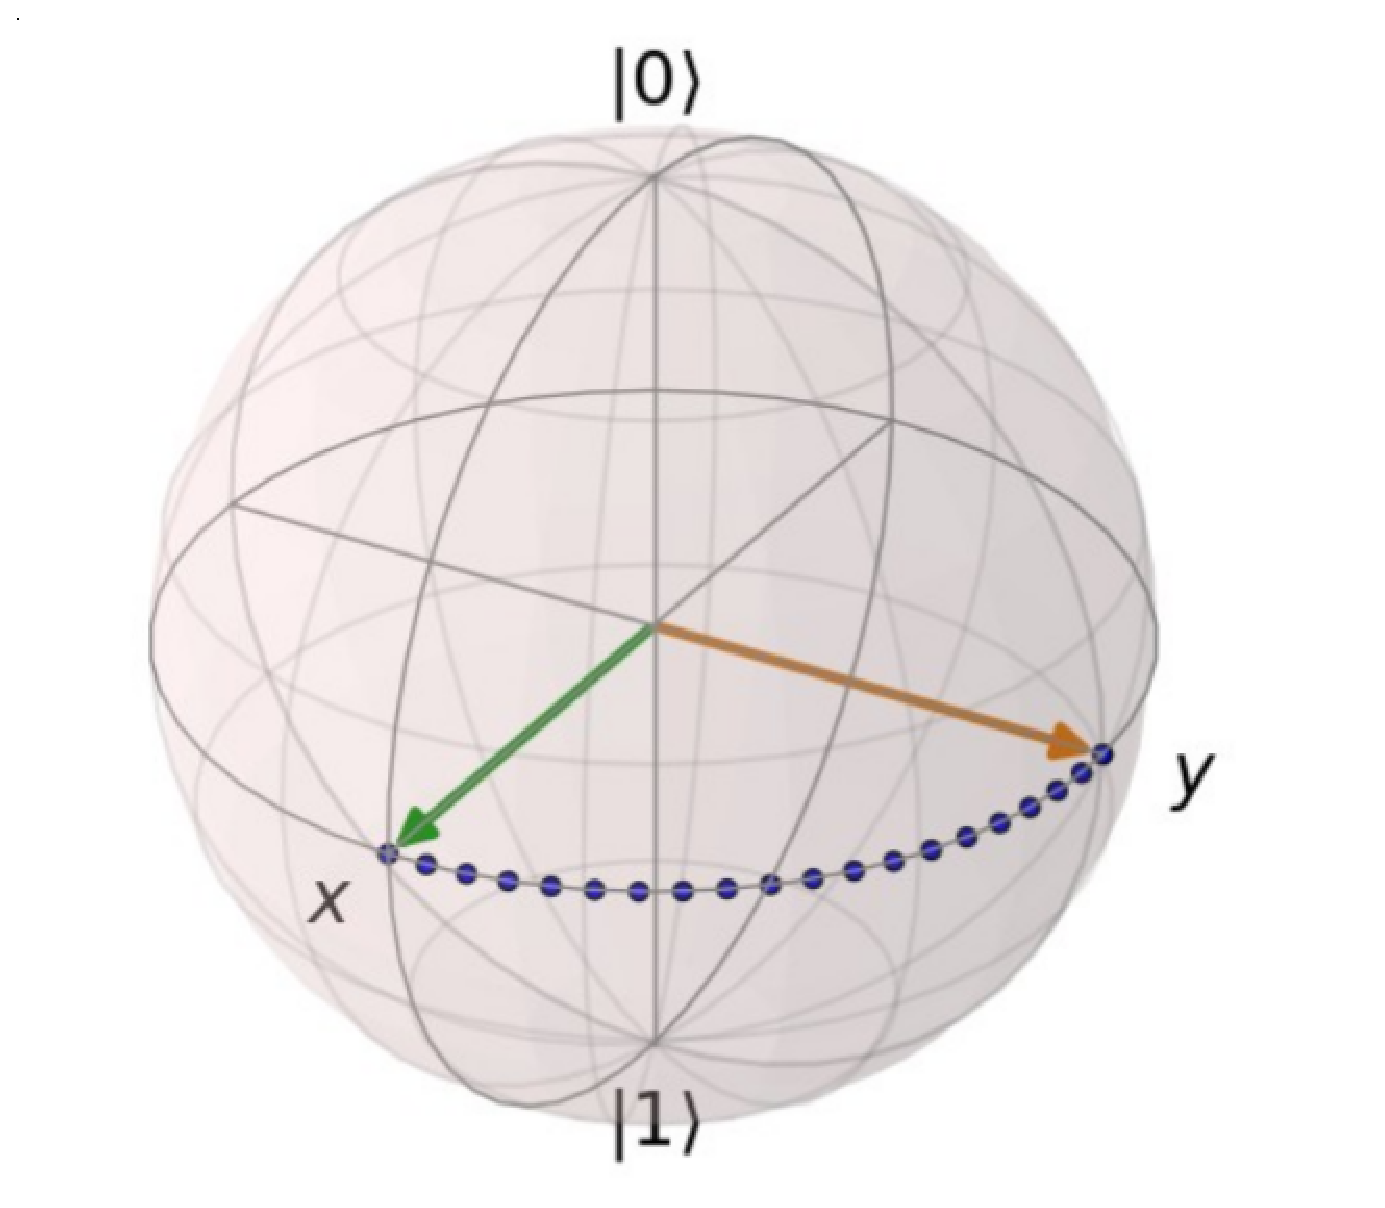
\includegraphics[scale=0.21]{images/s_gate.eps}
  \vspace{1mm}
  \caption{S gate rotation visualized on the Bloch sphere.}
  \label{fig:s_bloch}
\end{figure}

\section{Measurement}
Measuring a quantum state \ket{\psi} \emph{collapses} the quantum superposition to a classical state \ket{j} (which in the computational basis is \ket{0} or \ket{1}). The state \ket{\psi} has ``disappeared" and all that is left is the classical state \ket{j}. The probabilistic result of a measurement of a quantum state $\ket{\psi} = \alpha\ket{0} + \beta\ket{1}$ can be calculated based on the probability amplitudes:
\begin{equation}
\begin{aligned}
  P(\ket{0}) &= \left|\alpha\right|^2 \\
  P(\ket{1}) &= \left|\beta\right|^2.
\end{aligned}
\end{equation}
Consider the following simple single-qubit circuit:

\begin{figure}[ht]
\[
  \Large{
    \Qcircuit @C=1em @R=0em {
    \push{\rule{0em}{1em}} & & \lstick{\ket{0}} & \gate{H} & \gate{Z} & \meter & \cw
    }
  }
\]
\caption{A simple quantum circuit. The output of measuring a qubit is a classical bit, which is distinguished from a qubit by drawing a double-line wire. A visualization of this circuit on the Bloch sphere can be seen in Figure~\ref{fig:gate_rotations}.}
\end{figure}
\noindent
We start with computing $H\ket{0} = \ket{+}$, followed by $Z\ket{+} = \frac{1}{\sqrt2}(\ket{0} - \ket{1})$ \, (or \ket{-}), and finally we measure, giving us a classical state \ket{j} and collapsing the state. Which state we will see is not determined in advance; the only thing we can say is that we will see \ket{j} with probability $|a_j|^2$:
\begin{equation}
\begin{aligned}
  P(\ket{0}) = \left|\dfrac{1}{\sqrt2}\right|^2 &= \dfrac{1}{2} \\
  P(\ket{1}) = \left|\dfrac{-1}{\sqrt2}\right|^2 &= \dfrac{1}{2}.
\end{aligned}
\end{equation}
Giving us equal probabilities of our state being measured as \ket{0} or \ket{1}.

\begin{figure}[ht]
  \centering
  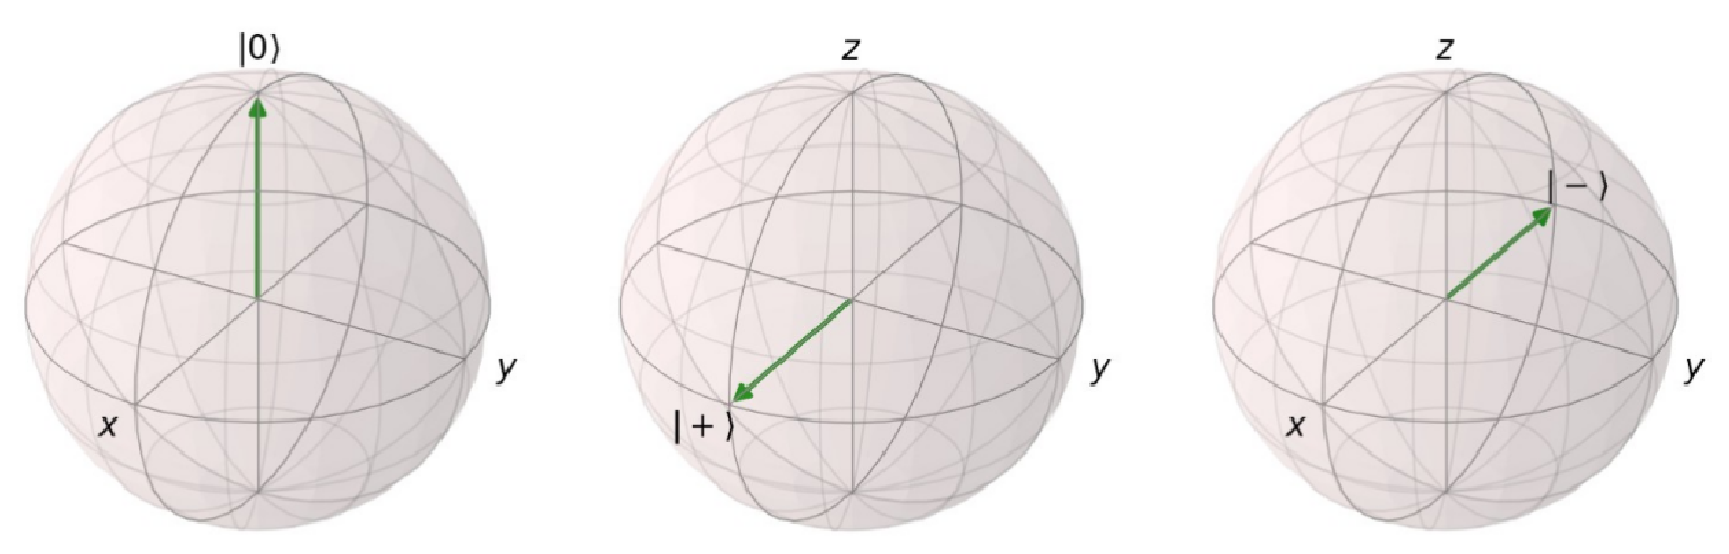
\includegraphics[scale=0.335]{images/simple_circuit.eps}
  \vspace{2mm}
  \caption{States of our qubit throughout the circuit from left to right: \ket{0} $\rightarrow$ $H$\ket{0} $\rightarrow$ $ZH$\ket{0}.}
  \label{fig:gate_rotations}
\end{figure}

\section{Vector Notation} \label{sec:matrix_notation}
Earlier we showed that we can represent a quantum state as
\begin{equation}
  \ket{\psi} = \alpha\ket{0} + \beta\ket{1}.
\end{equation}
The quantum states \ket{\psi}, \ket{0} and \ket{1} in the formula above are vectors. We define \ket{0} and \ket{1}, the computational basis states, as following:
\setlength\multicolsep{0pt}
\begin{equation}
\ket{0} = \qstatezero{}; \quad \ket{1} = \qstateone{}.
\end{equation}
\noindent
A quantum state has to be a normalized vector. In general, a qubit's state is a unit vector in a two-dimensional complex vector space. A $n$ qubit state has a $2^n$ dimensional \emph{Hilbert space}. We can consider a quantum state to be a linear combination of the computational basis states:
\begin{equation}
  \ket{\psi} = \alpha\qstatezero{} + \beta\qstateone{} = \begin{pmatrix}\alpha \\ \beta\end{pmatrix}.
\end{equation}
Single-qubit gates can then be represented by $2 \times 2$ unitary matrices:
\vspace*{-4mm}
\setlength\multicolsep{0pt}
\begin{multicols}{3}
  \[
    I = \igate{}
  \]
  \vfill
  \[
    X = \xgate{}
  \]
  \vfill
  \[
    Y = \ygate{}
  \]
\end{multicols}
\begin{multicols}{3}
  \[
    Z = \zgate{}
  \]
  \vfill
  \[
    S = \sgate{}
  \]
  \vfill
  \[
    H = \hgate{}
  \]
\end{multicols}
\bigskip
\noindent
Then a computation like $X$\ket{0} can be calculated by matrix vector multiplication:
\begin{equation}
X\ket{0} = \xgate{} \qstatezero{} = \qstateone{}.
\end{equation}
And we find that $X\ket{0} = \ket{1}$. Or, more general:
\begin{equation}
  X\begin{pmatrix}\alpha \\ \beta\end{pmatrix} = \begin{pmatrix}\beta \\ \alpha\end{pmatrix}.
\end{equation}

You can combine quantum gates by multiplying their matrices. For example, let's verify that $H$ is self-inverse by applying it to itself:
\begin{equation}
  H^2 = \hgate{} \hgate{} = \igate{} = I.
\end{equation}
The result is the identity gate, showing that the inverse of $H$ is indeed itself. It is also a \emph{Hermitian matrix}, because it is equal to its own conjugate transpose: $H = H^\dagger$.

\newpage

\chapter{Fundamentals: A Multi-Qubit World}
We can represent multiple qubit states using the \emph{Kronecker product}. Let $A$ be a $m \times n$ matrix and $B$ a $p \times q$ matrix, then
\begin{equation}
  A \otimes B =
    \begin{pmatrix}
      a_{11}B & \dots & a_{1n}B \\
      \vdots & \ddots & \vdots \\
      a_{m1}B & \dots & a_{mn}B \\
    \end{pmatrix},
\end{equation}
resulting in a $mp \times nq$ matrix. We can then represent the two qubit state \ket{00} as
\begin{equation}
  \ket{00} = \ket{0} \otimes \ket{0} = \qstatezero{} \otimes \qstatezero{} =
  \begin{pmatrix}
    1\qstatezero{} \\[13pt]
    0\qstatezero{}
  \end{pmatrix}
  =
  \begin{pmatrix}
    1 \\
    0 \\
    0 \\
    0
  \end{pmatrix}.
\end{equation}
Throughout this document we will use different kinds of notation for multiple qubits depending on context, all of which are equivalent: $\ket{00} = \ket{0}\!\ket{0} = \ket{0} \otimes \ket{0}$.
We can write a two qubit state as following in Dirac notation:
\begin{equation}
  \ket{ab} = \ket{a} \otimes \ket{b} = \alpha_{00}\ket{00} + \alpha_{01}\ket{01} + \alpha_{10}\ket{10} + \alpha_{11}\ket{11}.
\end{equation}
More generally, we say that a linear combination $\sum_{i} \alpha_i\ket{\psi_i}$ is a quantum state with states \ket{\psi_i} and amplitude $\alpha_i$ for state \ket{\psi_i}.

Note that the state vector of two qubits is twice as big as the state vector for one qubit. This is where some of the potential power of quantum computers comes from. With $n$ qubits you can represent $2^n$ states - the state space grows exponentially with the number of qubits, unlike classical bits. For multi-qubit states the rule remains that the state vector has to be normalized. For a $n$ qubit state:
\begin{equation}
  \sum_{i = 0}^{2^n-1} |\alpha_i|^2 = 1.
\end{equation}

\section{Quantum State Evolution}
Doing single-qubit operations on a multi-qubit state is possible by combining the identity and our single-qubit gate. Say we want to compute $H_1$\ket{0_0 0_1}. That is, put the second qubit through a Hadamard gate.\footnote{Note that when I say ``second" qubit, I'm talking about the most right, or least significant qubit. I will number them for this example but assume it from here on out.} To do so, the gate matrix's column width has to be equal to the quantum state vector's dimension. We can achieve this by taking the Kronecker product of the identity matrix and our single-qubit matrix (in this case $H$):
\begin{equation}
  H_1\ket{0_0 0_1} = (I_0 \otimes H_1)\ket{0_0 0_1}.
\end{equation}
Writing it out:
\begin{align}
  I_0 \otimes H_1 &=
  \igate{} \otimes \hgate{} \\
  &=
  \dfrac{1}{\sqrt2}
  \left[
  \igate{}
  \otimes
  \begin{pmatrix}
  1 & \phantom{-}1 \\
  1 & -1
  \end{pmatrix}
  \right] \\
  &= \dfrac{1}{\sqrt2}
  \begin{pmatrix}
  1 & \phantom{-}1 & 0 & \phantom{-}0 \\
  1 & -1 & 0 & \phantom{-}0 \\
  0 & \phantom{-}0 & 1 & \phantom{-}1 \\
  0 & \phantom{-}0 & 1 & -1 \\
  \end{pmatrix}.
\end{align}
Then we can put our \ket{00} state through it:
\begin{equation}
  \dfrac{1}{\sqrt2}
  \begin{pmatrix}
  1 & \phantom{-}1 & 0 & \phantom{-}0 \\
  1 & -1 & 0 & \phantom{-}0 \\
  0 & \phantom{-}0 & 1 & \phantom{-}1 \\
  0 & \phantom{-}0 & 1 & -1 \\
  \end{pmatrix}
  \begin{pmatrix}
  1 \\
  0 \\
  0 \\
  0
  \end{pmatrix}
  =
  \dfrac{1}{\sqrt2}
  \begin{pmatrix}
  1 \\
  1 \\
  0 \\
  0
  \end{pmatrix},
\end{equation}
which can also be written in Dirac notation as $\dfrac{1}{\sqrt2}(\ket{00} + \ket{01})$.

\section{Partial Measurement}
Say we measure the qubit \ket{q_0} in the following circuit:
\[
  \Large
  \Qcircuit @C=1em @R=0.5em @!R {
    \push{\rule{0em}{1.5em}} & & & & & \lstick{\ket{q_0} = \ket{0}} & \gate{H} & \meter & \cw \\
    \push{\rule{0em}{1.5em}} & & & & & \lstick{\ket{q_1} = \ket{0}} & \gate{H} & \qw & \qw \\
  }
\]
\noindent
First, we put both qubits in our state \ket{00} through a Hadamard gate. This puts it in the state
\begin{equation}
  (H \otimes H)\ket{00} = \dfrac{1}{2}(\ket{00} + \ket{01} + \ket{10} + \ket{11}).
\end{equation}
When we measure \ket{q_0} we have a 50/50 probability of getting a 0 or 1. Measuring \ket{q_0} collapses the state to one of the following states:
\begin{equation}
  \ket{\psi} = 
  \begin{cases}
  \begin{aligned}
    \dfrac{1}{\sqrt2}(\ket{\uline{0}0} + \ket{\uline{0}1}) & \text{ if } M(q_0) = 0 \\
    \dfrac{1}{\sqrt2}(\ket{\uline{1}0} + \ket{\uline{1}1}) & \text{ if } M(q_0) = 1
  \end{aligned}
  \end{cases}
\end{equation}
We have two possible states for $q_0$ after measurement: 0 or 1. Qubit \ket{q_1} will stay in superposition because we haven't measured it. Notice how the first qubits (underlined) in both states are the same. This makes sense, we've measured that one so we're certain of its state.

\section{Common Two-Qubit Gates}
\subsection{CNOT Gate}
The quantum gate controlled-\textsc{not} (\textsc{cnot}, sometimes called controlled-$X$) is comparable to a classical computer's \textsc{xor}, but it's reversible. This gate has two input qubits, the \emph{control} qubit and \emph{target} qubit. If the control qubit is set to 0, then the target qubit is left alone. If the control qubit is set to 1, then the target qubit is flipped. The circuit representation for \textsc{cnot} can be seen in Figure~\ref{fig:cnot_circuit}. Qubit \ket{q_0} represents the control qubit and \ket{q_1} represents the target qubit. It's essentially a Pauli X gate with a control qubit. \textsc{cnot} is Hermitian and belongs to the Clifford gates.

\begin{figure}[ht]
\centering
\begin{minipage}{.45\textwidth}
  \[
    \Large
    \Qcircuit @C=1em @R=0.5em @!R {
	  \push{\rule{0em}{1em}} & & \lstick{\ket{q_0}} & \ctrl{1} & \qw & \ctrl{1} & \qw \\
	  \push{\rule{0em}{1em}} & & \lstick{\ket{q_1}} & \targ & \qw & \gate{X} & \qw    \\
	}
  \]
  \caption{Two different circuit representations of \textsc{cnot}. We will use the left representation.}
  \label{fig:cnot_circuit}
\end{minipage}%
\hspace*{.05\textwidth}
\begin{minipage}{.45\textwidth}
  \[
    U_{CN} = \cnotgate{}
  \]
  \caption{Matrix representation of \textsc{cnot}.}
\end{minipage}
\end{figure}
\noindent
Let's look at an example of a \textsc{cnot} gate. Consider the following circuit:
\[
  \Large
  \Qcircuit @C=1em @R=0.5em @!R {
    \push{\rule{0em}{1.5em}} & & & & & \lstick{\ket{q_0} = \ket{0}} & \gate{X}  & \ctrl{1} & \qw & \qw\\
    \push{\rule{0em}{1.5em}} & & & & & \lstick{\ket{q_1} = \ket{0}} & \qw & \targ & \qw & \qw\\
  }
\]
First we put \ket{q_0} (the control qubit) in the \ket{1} state by applying an $X$ gate, giving us the state \ket{10}. Then we apply the \textsc{cnot} gate, giving
\begin{equation}
  \textsc{CNOT}\ket{10} = \cnotgate{}
  \begin{pmatrix}
  0 \\
  0 \\
  1 \\
  0
  \end{pmatrix}
  =
  \begin{pmatrix}
  0 \\
  0 \\
  0 \\
  1
  \end{pmatrix}
  =
  \ket{11}.
\end{equation}
The target qubit was flipped because the control qubit was set to \ket{1}, giving us \ket{11}.

\subsection{CZ Gate}
\textsc{cz}, or the controlled-$Z$ gate, acts in a similar way to other controlled gates. That is, do the operation on the target qubit if the control qubit is \ket{1}, otherwise do nothing. In \textsc{cz} the operation is the Pauli Z gate. \textsc{cz} is also Hermitian and belongs to the Clifford gates.
\begin{figure}[ht]
\[
  \Large
  \Qcircuit @C=1em @R=0.5em @!R {
    \push{\rule{0em}{1em}} & & \lstick{\ket{q_0}} & \ctrl{1} & \qw & \ctrl{1} & \qw \\
    \push{\rule{0em}{1em}} & & \lstick{\ket{q_1}} & \ctrl{-1} & \qw & \gate{Z} & \qw  \\
  }
\]
\caption{Two different circuit representations of \textsc{CZ}.}
\end{figure}

\subsection{Controlled Gates}
Controlled gates act on two or more qubits, where one or more qubits act as control for some operation. Generally, if $U$ is a gate that operates on single qubits with the following matrix representation:
\begin{equation}
  U =
  \begin{pmatrix}
  u_{00} & u_{01} \\
  u_{10} & u_{11} \\
  \end{pmatrix},
\end{equation}
then the controlled-$U$ gate is a gate that operates on two qubits where the first qubit serves as control. The general matrix representation of the controlled-$U$ then, if qubit 0 is the control and qubit 1 is the target, looks as following:
\begin{equation}
  C_U =
  \begin{pmatrix}
  1 & 0 & 0 & 0 \\
  0 & 1 & 0 & 0 \\
  0 & 0 & u_{00} & u_{01} \\
  0 & 0 & u_{10} & u_{11} \\
  \end{pmatrix}.
\end{equation}
\section{Toffoli Gate}
The Toffoli gate has three inputs and outputs (Figure \ref{fig:toffoli_circuit}), where two of the input qubits act as control bits. The third qubit is the target bit which is flipped if both control qubits are set to \ket{1}, otherwise it's left alone. For example, applying the Toffoli gate to the state \ket{110} flips the third qubit, resulting in the state \ket{111}.

\begin{figure}[ht]
  \[
    \Large
    \Qcircuit @C=0.54em @R=1em @!R {
      \push{\rule{0em}{1em}} & & & \lstick{a} & \ctrl{1} & \qw & a\\
      \push{\rule{0em}{1em}} & & & \lstick{b} & \ctrl{1} & \qw & b\\
      \push{\rule{0em}{1em}} & & & \lstick{c} & \targ & \qw & & & c \otimes ab\\
    }
  \]
  \caption{Circuit representation of the Toffoli gate, where $\otimes$ is addition modulo two.}
  \label{fig:toffoli_circuit}
\end{figure}
\noindent
The Toffoli, or controlled-controlled-X (\textsc{ccx}) gate can be represented by a $8 \times 8$ matrix:
\begin{equation}
  U_{CCX} =
  \begin{pmatrix}
  1 & 0 & 0 & 0 & 0 & 0 & 0 & 0\\
  0 & 1 & 0 & 0 & 0 & 0 & 0 & 0\\
  0 & 0 & 1 & 0 & 0 & 0 & 0 & 0\\
  0 & 0 & 0 & 1 & 0 & 0 & 0 & 0\\
  0 & 0 & 0 & 0 & 1 & 0 & 0 & 0\\
  0 & 0 & 0 & 0 & 0 & 1 & 0 & 0\\
  0 & 0 & 0 & 0 & 0 & 0 & 0 & 1\\
  0 & 0 & 0 & 0 & 0 & 0 & 1 & 0\\
  \end{pmatrix}.
\end{equation}

\section{Universal Gate Sets}
In classical systems the \textsc{nand} gate is a universal gate, meaning that any other gate can be represented as a combination of \textsc{nand} gates. In quantum computing there exist universal gate sets. A universal gate set requires the full Clifford and Pauli groups, and one or more non-Clifford gates.

We've seen the Pauli gates in Section \ref{pauli_gates}. On their own, Pauli gates have no interesting computational capabilities. The Clifford gates we've seen are $H$, $S$, \textsc{cnot} and \textsc{cz}. Clifford gates introduce the quantum phenomena superposition and entanglement. The Pauli and Clifford gates can be simulated efficiently by classical computers (\emph{Gottesman-Knill theorem}) - showing no increase in efficiency over classical computers.

The non-Clifford gates, which are required for universal quantum computing, cannot be simulated efficiently and are exponentially hard to simulate. Some non-Clifford gates are Toffoli, $T$ and the rotation gates $R_x$, $R_y$ and $R_z$ (which do arbitrary rotations around the axes). One set of universal gates is $\{H,\, T,\, \textsc{cnot}\}$.

\section{Entanglement}
Two qubits are \emph{entangled} if and only if the state of those two qubits can \emph{not be expressed as two individual states} (non-separable). Let's first take a look at a separable, or non-entangled state
\begin{equation} \label{eq:non_entangled_state}
  \ket{\psi} = \dfrac{1}{2}(\ket{00} + \ket{01} + \ket{10} + \ket{11}).
\end{equation}
This state can be separated and expressed as the following two individual states:
\begin{equation}
  \ket{\psi} = \dfrac{1}{\sqrt2}(\ket{0} + \ket{1}) \otimes \dfrac{1}{\sqrt2}(\ket{0} + \ket{1}).
\end{equation}
However, consider the state
\begin{equation} \label{eq:entangled_state}
  \ket{\psi} = \dfrac{1}{\sqrt2}(\ket{00} + \ket{11}).
\end{equation}
This is an entangled state, it cannot be expressed as two individual states. We say two qubits are entangled if they have \emph{nonzero concurrence}. The concurrence of a state can be calculated as following:
\begin{equation}
  C(\ket{\psi}) = 2|\alpha_{00}\alpha_{11} - \alpha_{01}\alpha_{10}|.
\end{equation}
We can check if our entangled state (\ref{eq:entangled_state}) is indeed entangled:
\begin{equation}
  C\left(\dfrac{1}{\sqrt2}(\ket{00} + \ket{11})\right) = 2\left|\dfrac{1}{\sqrt2}\left(\dfrac{1}{\sqrt2}\right)\right| = 1.
\end{equation}
It has a non-zero concurrence, so we can say it's entangled. How about the non-entangled state in \ref{eq:non_entangled_state}?
\begin{equation}
  C\left(\dfrac{1}{2}(\ket{00} + \ket{01} + \ket{10} + \ket{11})\right) = 2\left|\dfrac{1}{2}\left(\dfrac{1}{2}\right) - \dfrac{1}{2}\left(\dfrac{1}{2}\right)\right| = 0.
\end{equation}
A concurrence of 0, so it is not entangled.

\section{The Bell States} \label{sec:bell_states}
The \emph{Bell states} are four maximally entangled quantum states of two qubits:
\begin{align}
\ket{\Phi^+} &= \dfrac{1}{\sqrt2}(\ket{00} + \ket{11}) \\
\ket{\Phi^-} &= \dfrac{1}{\sqrt2}(\ket{00} - \ket{11}) \\
\ket{\Psi^+} &= \dfrac{1}{\sqrt2}(\ket{01} + \ket{10}) \\
\ket{\Psi^-} &= \dfrac{1}{\sqrt2}(\ket{01} - \ket{10}).
\end{align}
We can create a Bell state with the following circuit:
\[
  \Large
  \Qcircuit @C=0.5em @R=0.5em @!R {
    \push{\rule{0em}{1em}} & \ar@{.}[]+<4.75em,0.5em>;[d]+<4.75em,-1em> & & & & & & & & \lstick{\ket{q_0} = \ket{0}} & \qw & \qw & \gate{H} & \qw & \qw \ar@{.}[]+<0em,0.5em>;[d]+<0em,-1em> & \qw & \ctrl{1} & \qw & \qw & \qw \ar@{.}[]+<-0.7em,0.5em>;[d]+<-0.7em,-1em> \\
    \push{\rule{0em}{1em}} & & & & & & & & & \lstick{\ket{q_1} = \ket{0}} & \qw & \qw & \qw & \qw & \qw & \qw &\targ & \qw & \qw & \qw \\
    & \hspace{9.7em} \ket{\psi_0} & \hspace{15.3em} \ket{\psi_{1}} & \hspace{19.4em} \ket{\psi_{2}}
  }
\]
\vspace*{2mm}

\noindent
We start with our state \ket{00} at \ket{\psi_0}. We put \ket{q_0} through a Hadamard gate, giving us the state $\frac{1}{\sqrt2}(\ket{00} + \ket{10})$ at \ket{\psi_1}. Finally we \textsc{cnot} that state giving us the final Bell state $\ket{\Phi^+} = \frac{1}{\sqrt2}(\ket{00} + \ket{11})$ at \ket{\psi_2}.

The significance of Bell states becomes apparent when we start measuring qubits of a Bell state. Take the circuit we used before to create the Bell state $\frac{1}{\sqrt2}(\ket{00} + \ket{11})$ and measure both qubits.
\[
  \Large
  \Qcircuit @C=1em @R=0.5em @!R {
    \push{\rule{0em}{1em}} & & & & & & \lstick{\ket{q_0} = \ket{0}} & \gate{H} & \ctrl{1} & \meter & \cw  \\
    \push{\rule{0em}{1em}} & & & & & & \lstick{\ket{q_1} = \ket{0}} & \qw & \targ & \meter & \cw \\
  }
\]
You will find that the measurement results are correlated:
\begin{equation}
\begin{gathered}
M(q_1) = 0 \text{ if } M(q_0) = 0 \\
M(q_1) = 1 \text{ if } M(q_0) = 1
\end{gathered}
\end{equation}
If you measure \ket{q_0} to be 0, \ket{q_1} will also be 0 and vice versa. Note that in our example entangled state they correlate as being equal, but for the entangled state $\frac{1}{\sqrt2}(\ket{01} + \ket{10})$ they correlate as being opposites (measuring \ket{q_0} as 0 means \ket{q_1} will be 1).

\section{Greenberger-Horne-Zeilinger State}
A Greenberger-Horne-Zeilinger (GHZ) state is a certain type of entangled state. It is a $M > 2$ system state:
\begin{equation}
\ket{\textsc{GHZ}} = \dfrac{\ket{0}^{\otimes M} + \ket{1}^{\otimes M}}{\sqrt2},
\end{equation}
where $\ket{j}^{\otimes M}$ means the Kronecker product with itself $M$ times. For example $M = 3$:
\begin{equation}
\ket{\textsc{GHZ}} = \dfrac{\ket{000} + \ket{111}}{\sqrt2}.
\end{equation}
GHZ states are used for example in cryptography for secret sharing.
\begin{figure}[ht]
\[
  \Large
  \Qcircuit @C=1em @R=0.5em @!R {
  	\push{\rule{0em}{1em}} & & \lstick{\ket{0}} & \gate{H} & \ctrl{1} & \ctrl{2} & \qw  \\
	\push{\rule{0em}{1em}} & & \lstick{\ket{0}} & \qw & \targ & \qw & \qw \\
	\push{\rule{0em}{1em}} & & \lstick{\ket{0}} & \qw & \qw &  \targ & \qw \\
  }
\]
\caption{Circuit creating a three-qubit GHZ state.}
\label{fig:ghz_3}
\end{figure}

\section{Calculating Parity}
Parity checking is one of the simplest forms of error detecting code. It tells us if the number of ones in a set of bits is even or odd. For example, 001 has a parity of 1 (odd) and 110 has a parity of 0 (even). We introduce a quantum algorithm for calculating the parity of an $n$-qubit state. For this example we'll determine the parity of a two-qubit state. Consider the circuit in Figure~\ref{fig:parity_circuit}. We will calculate the parity of \ket{q_0}\ket{q_1} with \ket{q_2}.
\begin{figure}[ht]
  \[
  \Large
  \Qcircuit @C=1em @R=0.5em @!R {
    \push{\rule{0em}{1em}} & & & & & \lstick{\ket{q_0} = \ket{0}} & \gate{H} & \ctrl{2} & \qw & \qw & \qw \\
    \push{\rule{0em}{1em}} & & & & & \lstick{\ket{q_1} = \ket{0}} & \gate{H} & \qw & \ctrl{1} & \qw & \qw \\
    \push{\rule{0em}{1em}} & & & & & \lstick{\ket{q_2} = \ket{0}} & \qw & \targ &  \targ & \meter & \cw \\
  }
  \]
  \caption{Circuit for calculating parity: $\textsc{cnot}_{1,2}\textsc{cnot}_{0,2}H_1H_0\ket{000}$.}
  \label{fig:parity_circuit}
\end{figure}

We start with putting \ket{q_0} and \ket{q_1} in an arbitrary superposition. In this case we apply a Hadamard gate to both qubits, giving us the state
\begin{equation}
  \ket{\psi} = \dfrac{1}{2}(\ket{000} + \ket{010} + \ket{100} + \ket{110}).
\end{equation}
Then we apply a $\textsc{cnot}_{0,2}$ operation, giving
\begin{equation}
  \ket{\psi} = \dfrac{1}{2}(\ket{000} + \ket{010} + \ket{101} + \ket{111}),
\end{equation}
and a $\textsc{cnot}_{1,2}$:
\begin{equation}
  \ket{\psi} = \dfrac{1}{2}(\ket{000} + \ket{011} + \ket{101} + \ket{110}).
\end{equation}
If you look closely at this state, you can see that \ket{q_2} corresponds to the parity of \ket{q_0}\ket{q_1}. We have essentially calculated the parities of all possible states of \ket{q_0}\ket{q_1} in parallel. However, we cannot observe a quantum state to extract all the possible states' information. We are limited to measuring one outcome. When we measure \ket{q_2} the state partially collapses leaving only the states with parity $q_2$. Let's take a look at the possible states after measuring \ket{q_2}:
\begin{equation}
\ket{\psi} = 
\begin{cases}
\begin{aligned}
\dfrac{1}{\sqrt2}(\ket{00} + \ket{11}) \otimes \ket{0} & \text{ if } M(q_2) = 0 \\
\dfrac{1}{\sqrt2}(\ket{01} + \ket{10}) \otimes \ket{1} & \text{ if } M(q_2) = 1
\end{aligned}
\end{cases}
\end{equation}
Measuring a 0 leaves us with even parity states and measuring a 1 leaves us with odd parity states. \ket{00} and \ket{11} have even parity ($q_2 = 0$), \ket{01} and \ket{10} have odd parity ($q_2 = 1$).

\section{Quantum Teleportation}
Quantum teleportation it a technique for moving arbitrary quantum states around. It uses an \emph{EPR pair} (a pair of qubits that is in a Bell state) that is shared between the sender and receiver. Note that it is impossible to clone a qubit state. This is referred to as the \emph{no-cloning theorem}. Quantum teleportation works as following: Alice and Bob generate an EPR pair and both take one qubit before they get separated. Alice wants to deliver a qubit \ket{\phi}, whose state is unknown, to Bob. Alice interacts the qubit \ket{\phi} with her half of the EPR pair, and then measures the two qubits in her possession. At this point, Alice's qubits are in one of the four classical states 00, 01, 10 or 11. She sends this information to Bob. Bob then performs one of four operations on his half of the EPR pair, recovering Alice's quantum state \ket{\phi}.

\begin{figure}[ht]
  \[
  \Large
  \Qcircuit @C=1em @R=0.5em @!R {
	\push{\rule{0em}{1em}} & & & & \lstick{\ket{q_0} = \ket{\phi}} \ar@{.}[]+<0.55em,0.5em>;[d]+<0.55em,-3em> & \qw & \qw \ar@{.}[]+<0.9em,0.5em>;[d]+<0.9em,-3em> & \ctrl{1} \ar@{.}[]+<0.9em,0.5em>;[d]+<0.9em,-3em> &\gate{H} \ar@{.}[]+<1.2em,0.5em>;[d]+<1.2em,-3em> & \meter \ar@{.}[]+<1.5em,0.5em>;[d]+<1.5em,-3em> & \cw & \control \cw 
	\ar@{.}[]+<1.2em,0.5em>;[d]+<1.2em,-3em> \\
	\push{\rule{0em}{1em}} & & & & \lstick{\ket{q_1} = \ket{0}} & \gate{H} & \ctrl{1} & \targ & \qw &\meter & \control \cw & \cwx \\
	\push{\rule{0em}{1em}} & & & & \lstick{\ket{q_2} = \ket{0}} & \qw & \targ & \qw &\qw & \qw & \gate{X} \cwx & \gate{Z} \cwx &\rstick{\ket{\phi}} \qw \\
	& \hspace{7.3em} \ket{\psi_{0}} & \hspace{13.8em} \ket{\psi_{1}} & \hspace{15.6em} \ket{\psi_{2}} & \hspace{18.5em} \ket{\psi_{3}} & \hspace{20.9em} \ket{\psi_{4}} & \hspace{26.1em} \ket{\psi_{5}}
  }
  \]
  \vspace{3mm}
  \caption{Quantum circuit teleporting a quantum state \ket{\phi}.}
  \label{fig:teleportation}
\end{figure}
The circuit in Figure~\ref{fig:teleportation} teleports the unknown state $\ket{\phi} = \alpha\ket{0} + \beta\ket{1}$. We start at \ket{\psi_0} with the state
\ket{\phi}\ket{00}. Then we create an EPR pair with \ket{q_1}\ket{q_2}, where \ket{q_1} belongs to Alice and \ket{q_2} to Bob. This gives us the following state at \ket{\psi_1}:
\begin{equation}
  \ket{\psi_1} = \ket{\phi}\dfrac{1}{\sqrt2}(\ket{00} + \ket{11}),
\end{equation}
which we can rewrite as following
\begin{align}
\ket{\psi_1} &= \alpha\ket{0} + \beta\ket{1} \otimes \dfrac{1}{\sqrt2}(\ket{00} + \ket{11}) \\
&= \dfrac{1}{\sqrt2}\Big(\alpha\ket{0}(\ket{00} + \ket{11}) + \beta\ket{1}(\ket{00} + \ket{11})\Big).
\end{align}
Alice then sends her qubits through a $\textsc{cnot}_{0, 1}$ gate, obtaining
\begin{equation}
  \ket{\psi_2} = \dfrac{1}{\sqrt2}\Big(\alpha\ket{0}(\ket{00} + \ket{11}) + \beta\ket{1}(\ket{10} + \ket{01})\Big).
\end{equation}
She then sends \ket{q_0} through a Hadamard gate, giving
\begin{equation}
  \ket{\psi_3} = \dfrac{1}{2}\Big(\alpha(\ket{0} + \ket{1})(\ket{00} + \ket{11}) + \beta(\ket{0} - \ket{1})(\ket{10} + \ket{01})\Big).
\end{equation}
This state can be rewritten in the following way:
\begin{equation}
\begin{aligned}
  \ket{\psi_3} = \dfrac{1}{2}\Big(&\ket{00}(\alpha\ket{0} + \beta{\ket{1}}) \, + \ket{01}(\alpha\ket{1} + \beta\ket{0}) \\
  + \, &\ket{10}(\alpha\ket{0} - \beta\ket{1}) + \ket{11}(\alpha\ket{1} - \beta\ket{0})\Big).
\end{aligned}
\end{equation}
This expression breaks down in four terms. The first term has Alice's qubits in state \ket{00} and Bob's qubit in state $\alpha\ket{0} + \beta\ket{1}$, which is our original state \ket{\phi}. So in the case that Alice measures $M(q_0q_1) = 00$ at \ket{\psi_4}, Bob's qubit will be in state \ket{\phi}. Depending on Alice's measurement at \ket{\psi_4}, Bob may have to ``fix" his state to recover \ket{\phi} by applying the appropriate gate(s). For example, if Alice measures 00, Bob doesn't have to do anything. If Alice measures 01, Bob can fix his state by applying an $X$ gate. If Alice measures 10, Bob can fix his state by applying a $Z$ gate. And if Alice measures 11, Bob can fix his state by first applying an $X$ gate and then a $Z$ gate. After fixing his state, Bob ends up with Alice's state \ket{\phi} at \ket{\psi_5}.

Note that quantum teleportation does \emph{not} allow for faster than light communication. This is because Bob needs to be told of the result of Alice's measurements through a classical channel in order to complete the teleportation. Also note that we did not clone the quantum state \ket{\phi}, we merely moved it. Teleporting a state depends on the measurement and thus collapsing of the original state \ket{\phi}, so it never allows for cloning.

\chapter{Quantum Algorithms}
Quantum computers promise to solve problems intractable by classical computers. One application is quantum simulation. For example: simulating chemical processes, which are actually quantum processes. As Richard Feynman said: \say{\emph{Nature isn't classical, dammit, and if you want to make a simulation of nature, you'd better make it quantum mechanical.}} Other possible applications include optimization, cryptography and machine learning. There are a lot of efforts in trying to apply quantum computing, but many remain skeptic. We should assume no guarantees in the applications of quantum computers, but continue exploring the possibilities.

When a quantum computer can calculate something efficiently that a classical computer cannot calculate efficiently, we will have reached \emph{quantum supremacy}. The boundary of reaching this is around 50 qubits, when it becomes impossible to simulate a quantum computer. We have not yet reached quantum supremacy, but we are getting close to it. There have been found quantum algorithms which provide a speedup over classical algorithms, like Shor's algorithm for factoring integers and the Deutch-Jozsa algorithm for determining if a boolean function is balanced or unbalanced.

\section{Quantum Arithmetic}
Any classical circuit can be simulated by a quantum circuit. We can show this by creating quantum versions of classical arithmetic functions. One problem with simulating classical gates as quantum gates is that most of them are non-reversible. In quantum computing, it is required for gates to be reversible. This is often solved by adding an output qubit for every input qubit and an extra result qubit (Figure~\ref{fig:add_output_qubit}).
\begin{figure}[ht]
  \[
    \Large
    \Qcircuit @C=1em @R=0.5em {
      \push{\rule{0em}{1em}} & & \lstick{\ket{x}} & \multigate{1}{U_f} & \qw & \ket{x} \\
      \push{\rule{0em}{1em}} & & \lstick{\ket{y}} & \ghost{U_f} & \qw & & \hspace*{5.7mm} \ket{y \otimes f(x)}
    }
  \]
  \caption{Create output qubits for every input qubit in \ket{x} and store the result of $f(x)$ in \ket{y}. This transformation can be described as $U_f\ket{x}\!\ket{y} = \ket{x}\!\ket{y \otimes f(x)}$. The $\otimes$ symbol in this context means the binary sum (\textsc{xor}).}
  \label{fig:add_output_qubit}
\end{figure}
We can create a quantum half adder by creating sum and carry circuits, just like in classical computers. The truth table of the sum function $f_s(x)$ can be found in Figure \ref{fig:sum_truth_table}. We can implement this as a quantum circuit using \textsc{cnot} gates as seen in Figure \ref{fig:sum_quantum_circuit}.

\begin{figure}[ht]
  \begin{minipage}{.45\textwidth}
    \centering
    \begin{tabular}{c|c}
      $x_0$$x_1$ & $f_s(x)$ \\ \hline
      00 & 0 \\
      01 & 1 \\
      10 & 1 \\
      11 & 0 \\
    \end{tabular}
    \caption{Bit sum truth table.}
    \label{fig:sum_truth_table}
  \end{minipage}%
  \hspace*{.05\textwidth}
  \begin{minipage}{.45\textwidth}
    \[
      \Large
      \Qcircuit @C=1em @R=0.5em @!R {
        \push{\rule{0em}{1em}} & & \lstick{\ket{x_{0}}} & \ctrl{2} & \qw & \qw \\
        \push{\rule{0em}{1em}} & & \lstick{\ket{x_{1}}} & \qw & \ctrl{1} & \qw \\
        \push{\rule{0em}{1em}} & & \lstick{\ket{y}} & \targ &  \targ & \qw \\
      }
    \]
    \caption{Quantum circuit for summing two bits using two \textsc{cnot} gates.}
    \label{fig:sum_quantum_circuit}
    \end{minipage}
\end{figure}

To fully add two bits we need to account for the carry. The carry function $f_c(x)$ is 1 if and only if both inputs are 1 (Figure~\ref{fig:carry_truth_table}). This truth table corresponds directly to the Toffoli gate (Figure~\ref{fig:carry_quantum_circuit}).

\begin{figure}[ht]
  \begin{minipage}{.45\textwidth}
    \centering
    \begin{tabular}{c|c}
      $x_0$$x_1$ & $f_c(x)$ \\ \hline
      00 & 0 \\
      01 & 0 \\
      10 & 0 \\
      11 & 1 \\
    \end{tabular}
    \caption{Bit carry truth table.}
    \label{fig:carry_truth_table}
  \end{minipage}%
  \hspace*{.05\textwidth}
  \begin{minipage}{.45\textwidth}
    \[
      \Large
      \Qcircuit @C=1em @R=0.5em @!R {
        \push{\rule{0em}{1em}} & & \lstick{\ket{x_{0}}} & \ctrl{2} & \qw \\
        \push{\rule{0em}{1em}} & & \lstick{\ket{x_{1}}} & \ctrl{1} & \qw \\
        \push{\rule{0em}{1em}} & & \lstick{\ket{y}} & \targ & \qw \\
      }
    \]
    \caption{Quantum circuit for taking the carry of two bits implemented using a Toffoli gate.}
    \label{fig:carry_quantum_circuit}
  \end{minipage}
\end{figure}
\noindent
We can combine our sum and carry circuit into one, creating a quantum half adder.

\begin{figure}[ht]
  \[
  \Large
  \Qcircuit @C=1em @R=0.5em @!R {
    \push{\rule{0em}{1em}} & \lstick{\ket{x_0}} & \ctrl{3} & \ctrl{2} & \qw & \qw & \ket{x_0} \\
    \push{\rule{0em}{1em}} & \lstick{\ket{x_1}} & \ctrl{2} & \qw &  \ctrl{1} & \qw & \ket{x_1} \\
    \push{\rule{0em}{1em}} & \lstick{\ket{0}} & \qw & \targ & \targ & \qw & \ket{y_s} \\
    \push{\rule{0em}{1em}} & \lstick{\ket{0}} & \targ & \qw & \qw & \qw & \ket{y_c} \\
  }
  \]
  \caption{Quantum half adder. The sum ends up in \ket{y_s} and the carry in \ket{y_c}.}
  \label{fig:quantum_full_adder}
\end{figure}
\noindent
Let's check if this circuit works. Say we want to add $\ket{x_0} = \ket{1}$ and $\ket{x_1} = \ket{1}$. We would expect to get 0 as sum and 1 as carry. Our initial state is \ket{1100}. We apply a Toffoli gate, setting the carry qubit to 1: \ket{1101}. Then we set the sum qubit by doing a $\textsc{cnot}_{0,2}$ and a $\textsc{cnot}_{1,2}$ ending up with the state \ket{1101}. Measuring the sum and carry qubits gives $M(y_s) = 0$ and $M(y_c) = 1$, giving us what we expected and thus having done a quantum half addition of two qubits.

\section{Deutch-Jozsa Algorithm}
We have shown that we can simulate classical circuits on a quantum computer. This in itself isn't very impressive however, we could already do that on a classical computer. In this section we will describe an algorithm with quantum speedup. Consider the four single-bit operations identity, \textsc{not}, reset and set. 

\begin{figure}[ht]
  \centering
  \begin{multicols}{4}
    \captionof*{table}{\textbf{Identity}\\$f_i(x) = x$}
    \begin{tabular}{c|c}
    $x$ & $f_i(x)$ \\ \hline
    0 & 0 \\
    1 & 1 \\
    \end{tabular}

    \captionof*{table}{\textbf{NOT}\\$f_n(x) = \neg x$}
    \begin{tabular}{c|c}
    $x$ & $f_n(x)$ \\ \hline
    0 & 1 \\
    1 & 0 \\
    \end{tabular}

    \captionof*{table}{\textbf{Reset}\\$f_r(x) = 0$}
    \begin{tabular}{c|c}
    $x$ & $f_r(x)$ \\ \hline
    0 & 0 \\
    1 & 0 \\
    \end{tabular}

    \captionof*{table}{\textbf{Set}\\$f_s(x) = 1$}
    \begin{tabular}{c|c}
    $x$ & $f_s(x)$ \\ \hline
    0 & 1 \\
    1 & 1 \\
   \end{tabular}
  \end{multicols}

  \vspace{4mm}
  \caption{Truth tables for the four single-bit operations.}
  \label{fig:single_bit_operations}
\end{figure}
\noindent
Say we are faced with the following problem: we have a ``black box" with one of the four one-bit functions, but we're not told which one. Determine if the function is \emph{balanced} or \emph{unbalanced}. A balanced function is a function which returns the same amount of 0 and 1s it received as input, like identity and \textsc{not}. Unbalanced functions are functions which return a constant value, like reset and set. This is known as \emph{Deutch's problem} and is one of the first examples of a problem where there exists a quantum algorithm that is exponentially faster than any deterministic classical algorithm.

On a classical computer, to determine if the black box is balanced or unbalanced, we need to do two function calls. On a quantum computer, using the \emph{Deutch-Jozsa} algorithm, we can figure it out using one call to the black box. To use this algorithm for Deutch's problem we need to translate the four single-bit operations to the quantum world. The quantum circuits corresponding to each single-bit operation can be found in Figure~\ref{fig:single_bit_quantum_circuits}.
\vspace{-8mm}
\begin{figure}[ht]
  \centering
  \begin{multicols}{4}
    \[
      \Qcircuit @C=0.7em @R=0.8em @!R {
        \push{\rule{0em}{1em}} & & \lstick{\ket{x}} & \ctrl{1} & \qw \\
        \push{\rule{0em}{1em}} & & \lstick{\ket{y}} & \targ & \qw
      }
    \]
    \caption*{\textbf{Identity}\\$f_i(x) = x$}

    \[
      \Qcircuit @C=0.7em @R=0.5em @!R {
        \push{\rule{0em}{1em}} & & \lstick{\ket{x}} & \gate{X} & \ctrl{1} & \gate{X} & \qw \\
        \push{\rule{0em}{1em}} & & \lstick{\ket{y}} & \qw & \targ & \qw & \qw
      }
    \]
    \caption*{\textbf{NOT}\\$f_n(x) = \neg x$}

    \[
      \Qcircuit @C=0.7em @R=0.8em @!R {
        \push{\rule{0em}{1em}} & & & & & \lstick{\ket{x}} & \qw & \qw & \ghost{X} \\
        \push{\rule{0em}{1em}} & & & & & \lstick{\ket{y}} & \qw & \qw & \ghost{X}
      }
    \]
    \caption*{\textbf{Reset}\\$f_r(x) = 0$}
    
    \[
      \Qcircuit @C=0.7em @R=0.5em @!R {
        \push{\rule{0em}{1em}} & & \lstick{\ket{x}} & \qw & \qw \\
        \push{\rule{0em}{1em}} & & \lstick{\ket{y}} & \gate{X} & \qw
      }
    \]
    \caption*{\textbf{Set}\\$f_s(x) = 1$}
  \end{multicols}

  \vspace{3mm}
  \caption{Quantum circuit representation of the four single-bit operations.}
  \label{fig:single_bit_quantum_circuits}
\end{figure}

\noindent
With these definitions we can start using the Deutch-Jozsa algorithm to efficiently determine what kind of function our black box is. The circuit to do so is described in Figure~\ref{fig:deutch_jozsa_circuit}. In this circuit, $U_f$ refers to our black box function, or as it is sometimes also called, \emph{oracle}.

\begin{figure}[ht]
  \[
    \Large
    \Qcircuit @C=1em @R=1em @!R {
      \push{\rule{0em}{1em}} & & & \lstick{x: \ket{0}} & \gate{H} & \multigate{1}{U_f} & \gate{H} & \meter & \cw \\
      \push{\rule{0em}{1em}} & & & \lstick{y: \ket{1}} & \gate{H} & \ghost{U_f} &  \qw & \qw & \qw
    }
  \]
  \caption{Quantum circuit to determine if $f$ is a balanced or unbalanced function using the Deutch-Jozsa algorithm. $U_f$ is the quantum circuit which transforms \ket{x}\ket{y} to \ket{x}\ket{y \otimes f(x)}.}
  \label{fig:deutch_jozsa_circuit}
\end{figure}
We can try it out by trying to determine if the identity function $f_i(x) = x$ is balanced or unbalanced. We start with putting \ket{x} and \ket{y} through a Hadamard gate:
\begin{equation}
  \ket{\psi} = \dfrac{1}{2}(\ket{00} - \ket{01} + \ket{10} - \ket{11}).
\end{equation}
We evaluate our identity function using by applying $U_f$:
\begin{equation}
\begin{aligned}
\ket{\psi} = \dfrac{1}{2}\big(&\ket{0}\!\ket{0 \otimes f_i(0)} - \ket{0}\!\ket{1 \otimes f_i(0)} \\
+\, &\ket{1}\!\ket{0 \otimes f_i(1)} - \ket{1}\!\ket{1 \otimes f_i(1)}\big).
\end{aligned}
\end{equation}
This state contains information about both $f_i(0)$ and $f_i(1)$! We have essentially evaluated two values of $f_i(x)$ simultaneously, a feature known as \emph{quantum parallelism}. Actually applying the function $f_i(x)$, which as we can see in Figure~\ref{fig:single_bit_quantum_circuits} is just a $\textsc{cnot}_{0, 1}$, gives us the state
\begin{equation}
  \ket{\psi} = \dfrac{1}{2}(\ket{00} - \ket{01} + \ket{11} - \ket{10}).
\end{equation}
Finally we apply another Hadamard gate on \ket{x}:
\begin{equation}
\begin{aligned}
  \ket{\psi} = \dfrac{1}{2\sqrt2}(&\ket{00} + \ket{10} - \ket{01} - \ket{11} \\
  + \, &\ket{01} - \ket{11} - \ket{00} + \ket{10})
\end{aligned}
\end{equation}
\vspace*{-7mm}
\begin{align}
  \phantom{\ket{\psi}} &= \dfrac{1}{2\sqrt2}(\ket{10} + \ket{10} - \ket{11} - \ket{11}) \\
  &= \dfrac{1}{\sqrt2}(\ket{10} - \ket{11}).
\end{align}
We end up with the final state $\frac{1}{\sqrt2}(\ket{10} - \ket{11})$ before measurement. We can see from this state that $M(x) = 1$. Curiously, the following measurement outcomes apply:
\begin{equation}
\begin{aligned}
\ket{0_x} \otimes \dfrac{1}{\sqrt2}(\ket{0_y} - \ket{1_y}) & \, \text{ if } \, f(0) = f(1) \\
\ket{1_x} \otimes \dfrac{1}{\sqrt2}(\ket{0_y} - \ket{1_y}) & \, \text{ if } \, f(0) \not= f(1)
\end{aligned}
\end{equation}
That is, we get $M(x) = 1$ if $f(0) \not= f(1)$, which means $f$ is a balanced function. Likewise, we get $M(x) = 0$ if $f(0) = f(1)$, which means $f$ is an unbalanced function. Since we got a measurement of 1 for $f_i$, and given the fact that the identity operation is balanced, we can say that we effectively determined that $f_i$ is a balanced function with one call to the black box.

\section{Quantum Fourier Transform}
An important operation in classical computing and quantum computing as we will see is the \emph{Fourier transform}. The Fourier transform transforms a function $f(t)$ in the time domain to another function $F(x)$ in the frequency domain. The opposite (transforming a function in the frequency domain to a function in the time domain) can be achieved by applying the \emph{inverse} Fourier transform. Consider the sinusoidal function $f(t) = \cos(t)$. Figure~\ref{fig:cos_time_graph} graphs this function in the time domain, with time on the $x$ axis and amplitude on the $y$ axis. Applying the Fourier transform on this function gives us a function of the frequency domain, as seen in Figure~\ref{fig:cos_freq_graph}.
\begin{figure}[ht]
  \centering
  \begin{multicols}{2}
    \begin{tikzpicture}
      \begin{axis}[
        title={$\cos(t)$},
        xlabel={$t$},
        axis lines = middle,
        xmax=2*pi,
        xmin=-2*pi,
        height=5cm,
        width=7cm,
        ymin=-1,
        ymax=1,
        xticklabels={$-2\pi$, , $-\pi$, , 
            , $\pi$, , $2\pi$},
        xtick={-6.28318, -4.7123889, -3.14159, -1.5708, 1.5708, 3.14159, 4.7123889, 6.28318}
      ]
         \addplot[red, domain=-2*pi:2*pi, samples=1000]{ cos(deg(x)) };
       \end{axis}
     \end{tikzpicture}
     \caption{Time domain plot of $\cos(t)$.}
     \label{fig:cos_time_graph}
     
     \begin{tikzpicture}
       \begin{axis}[
         title={$F(\cos(t))$},
         xlabel={$x$},
         axis lines=middle,
         height=5cm,
         width=6cm,
         xmax=2,
         xmin=-2,
         ymin=0,
         ymax=2
       ]
         \addplot[ycomb, blue, mark=, thick, mark=*] coordinates {
           (1, 1) (-1, 1)
         };
       \end{axis}
     \end{tikzpicture}
     \caption{Frequency domain plot of $F(\cos(t))$.}
     \label{fig:cos_freq_graph}
   \end{multicols}
\end{figure}

The Fourier transform is a very useful tool in computer science, used for example in signal processing. The signal shown in Figure~\ref{fig:cos_time_graph} is a continuous signal, meaning it is assumed to extend to infinity. Computers however can only deal with finite, non-continuous signals. This means we have to discretize the continuous function into discrete counterparts as seen in Figure~\ref{fig:cos_discrete_time_graph}. We can then transform the discrete signal using the \emph{discrete Fourier transform}.
\begin{figure}[ht]
  \centering
  \begin{tikzpicture}
    \begin{axis}[
      title={$\cos(t)$},
      xlabel={$t$},
      axis lines = middle,
      xmax=2*pi,
      xmin=-2*pi,
      height=5cm,
      width=8cm,
      ymin=-1,
      ymax=1,
      xticklabels={$-2\pi$, , $-\pi$, , , $\pi$, , $2\pi$},
      xtick={-6.28318, -4.7123889, -3.14159, -1.5708, 1.5708, 3.14159, 4.7123889, 6.28318}
    ]
      \addplot[ycomb, red, domain=-2*pi:2*pi, samples=25, mark=*, thick]{ cos(deg(x)) };
      \addplot[red, domain=-2*pi:2*pi, samples=1000, draw]{ cos(deg(x)) };
    \end{axis}
  \end{tikzpicture}
  \caption{Discretized counterpart of the continuous function $\cos(t)$. Each dot represents a sample of the signal. The time interval between the samples is called the sampling interval.}
  \label{fig:cos_discrete_time_graph}
\end{figure}  

The discrete Fourier transform can be thought of as a linear operation. This means we can map a $N$-dimensional state vector to another $N$-dimensional state vector by a $N \times N$ matrix $F_N$. For a $n$ qubit state $N$ is equal to $2^n$. Such transformation may be written as
\begin{equation}
  \ket{x} = \sum_{j=0}^{N-1}x_j\ket{j} \longrightarrow \sum_{k=0}^{N-1}y_k\ket{k},
\end{equation} 
where the amplitudes $y_k$ are the discrete Fourier transform of the amplitudes $x_j$. In other words, the quantum Fourier transform (QFT) transforms the computational basis states as following
\begin{equation} \label{eq:qft}
  F_N\ket{j} = \dfrac{1}{\sqrt N}\sum_{k=0}^{N-1}e^{2\pi i jk/N}\ket{k}.
\end{equation}
Note that this is the equivalent of a classical \emph{inverse} discrete Fourier transform. The quantum Fourier transform (QFT) has the same effect as the classical inverse Fourier transform and vice versa. The quantum Fourier transform provides an exponential speedup over the classical fast Fourier transform algorithm.

We have already seen and used the QFT on a single qubit. The unitary matrix of the QFT on one qubit is the Hadamard gate:
\begin{equation}
  F_2 = H = \hgate.
\end{equation}
For a multi-qubit system it becomes a bit more involved. To describe the circuit for the $n$-qubit QFT we need the Hadamard and controlled phase gate, which we will write as $R_k$ where
\begin{equation}
  R_k = \begin{pmatrix}
    1 & 0 \\
    0 & e^{2\pi i/2^k}
  \end{pmatrix}.
\end{equation}
The circuit for a QFT on 3 qubits can be seen in Figure~\ref{fig:quantum_3_qubit_fourier_circ}. Note that $S = R_2$ and $T = R_3$. The crossed gate at the end is the swap gate, which swaps two qubits. The order of qubits has to be reversed at the end of a QFT to get the correct order as result. Note that inverting the circuit by reversing the order of the gates and taking the inverse $U^\dagger$ of each gate $U$ gives an equally efficient circuit for the inverse quantum Fourier transform $F_N^\dagger$.

\begin{figure}[ht]
  \[
    \Large
    \Qcircuit @C=1em @R=0.5em @!R {
      \push{\rule{0em}{1em}} & & \lstick{\ket{x_0}} & \gate{H} & \gate{S} & \gate{T} & \qw & \qw & \qw & \qswap & \qw \\
      \push{\rule{0em}{1em}} & & \lstick{\ket{x_1}} & \qw & \ctrl{-1} & \qw & \gate{H} & \gate{S} & \qw & \qw \qwx & \qw \\
      \push{\rule{0em}{1em}} & & \lstick{\ket{x_2}} & \qw & \qw & \ctrl{-2} & \qw & \ctrl{-1} & \gate{H} & \qswap \qwx & \qw \\
    }
  \]
  \caption{Quantum Fourier transform on 3 qubits.}
  \label{fig:quantum_3_qubit_fourier_circ}
\end{figure}
\noindent
The matrix of a QFT can be written out using $\omega = e^{2\pi i/N}$. For 3 qubits, where $N = 8$:
\begin{equation}
  F_N = \dfrac{1}{\sqrt N}
  \begin{pmatrix}
    1 & 1 & 1 & 1 & 1 & 1 & 1 & 1 \\
    1 & \omega^1 & \omega^2 & \omega^3 & \omega^4 & \omega^5 & \omega^6 & \omega^7 \\
    1 & \omega^2 & \omega^4 & \omega^6 & 1 & \omega^2 & \omega^4 & \omega^6 \\
    1 & \omega^3 & \omega^6 & \omega^1 & \omega^4 & \omega^7 & \omega^2 & \omega^5 \\
    1 & \omega^4 & 1 & \omega^4 & 1 & \omega^4 & 1 & \omega^4 \\
    1 & \omega^5 & \omega^2 & \omega^7 & \omega^4 & \omega^1 & \omega^6 & \omega^3 \\
    1 & \omega^6 & \omega^4 & \omega^2 & 1 & \omega^6 & \omega^4 & \omega^2 \\
    1 & \omega^7 & \omega^6 & \omega^5 & \omega^4 & \omega^3 & \omega^2 & \omega^1 \\
  \end{pmatrix}.
\end{equation}
A more general circuit of the QFT for a $n$ qubit state is described below in Figure~\ref{fig:quantum_fourier_circ}.

\begin{figure}[ht]
  \begin{adjustwidth}{-2.5cm}{-2.5cm}
    \[
      \Qcircuit @C=0.8em @R=0.5em @!R {
        \push{\rule{0em}{1em}} & & \lstick{\ket{x_0}} & \gate{H} & \gate{R_2} & \qw & \dots & & \gate{R_{n-1}} & \gate{R_n} & \qw & \qw & \qw & \qw & \qw & \qw & \qw & \qw & \qw & \qw & \qw & \qw & \qw \\
        \push{\rule{0em}{1em}} & & \lstick{\ket{x_1}} & \qw & \ctrl{-1} & \qw & \dots & & \qw & \qw & \gate{H} & \qw & \dots & & \gate{R_{n-2}} & \gate{R_{n-1}} & \qw & \dots & & \qw & \qw & \qw & \qw \\
        \rstick{\vdots} & & & & \vdots & & & & & & & & & & & \\
        \push{\rule{0em}{1em}} & & \lstick{\ket{x_{n - 1}}} & \qw & \qw & \qw & \qw & \qw & \ctrl{-3} & \qw & \qw & \qw & \qw & \qw & \ctrl{-2} & \qw & \qw & \dots & & \gate{H} & \gate{R_2} & \qw & \qw \\
        \push{\rule{0em}{1em}} & & \lstick{\ket{x_n}} & \qw  & \qw & \qw & \qw & \qw & \qw & \ctrl{-4} & \qw & \qw & \qw & \qw & \qw & \ctrl{-3} & \qw & \dots & & \qw & \ctrl{-1} & \gate{H} & \qw \\
      }
    \]
  \end{adjustwidth}
  \caption{Quantum Fourier transform on $n$ qubits. Swap gates required to get the correct order at the end are omitted.}
  \label{fig:quantum_fourier_circ}
\end{figure}
The result of the Fourier transform of the original state is stored in the amplitudes. Remember however that these amplitudes cannot be extracted. Thus there is no way of determining the Fourier transform of the original state using the QFT\@. Even though we can't extract the transformed values after a QFT, the QFT has its use in quantum algorithms like Shor's algorithm for factoring integers and the quantum phase estimation algorithm.

\newpage

\section{Quantum Phase Estimation Algorithm}
The quantum phase estimation algorithm (QPE) is a quantum algorithm to estimate the phase of an eigenvector of a unitary operation. Say we prepare an eigenstate \ket{u} of a unitary operator $U$, where $U\!\ket{u} = e^{2\pi i \varphi}\ket{u}$ and the value of $\varphi$ is unknown ($0 \le \varphi \le 1$). The goal is to estimate the value of $\varphi$ when we don't necessarily know $U$ or \ket{u}, but have available black boxes capable of preparing \ket{u} and applying controlled-$U$ operations.

\begin{figure}[ht]
  \[
    \Large
    \Qcircuit @C=0.9em @R=0.5em @!R {
      \push{\rule{0em}{1em}} & & \lstick{\ket{0}} & \gate{H} & \qw & \qw & \qw & \dots & & \ctrl{4} & \multigate{3}{\,F^\dagger_n\,} & \qw & \meter & \cw \\
      \rstick{\vdots} & & & \vdots & & & & & & & & & \vdots \\
      \push{\rule{0em}{1em}} & & \lstick{\ket{0}} & \gate{H} & \qw & \ctrl{2} & \qw & \dots & & \qw & \ghost{\,F^\dagger_n\,} & \qw & \meter & \cw \\
      \push{\rule{0em}{1em}} & & \lstick{\ket{0}} & \gate{H} & \ctrl{1} &  \qw & \qw & \dots & & \qw & \ghost{\,F^\dagger_n\,} & \qw & \meter & \cw \\
      \push{\rule{0em}{1em}} & & \lstick{\ket{u}} & \qw {/^m} & \gate{U^{2^0}} & \gate{U^{2^1}} & \qw & \dots & & \gate{U^{2^{n-1}}} & \qw & \qw & \qw & \qw \\
    }
  \]
  \caption{Quantum phase estimation circuit, where $F^\dagger_n$ represent the inverse quantum Fourier transform on $n$ qubits. The '/' denotes a register of $m$ qubits.}
  \label{fig:phase_estimation_circ}
\end{figure}

The circuit for the QPE algorithm found in Figure~\ref{fig:phase_estimation_circ} consists of two registers. The upper $n$ qubits comprise the first register which will be used to calculate the estimate of $\varphi$. The size of the first register can be chosen based on two factors: accuracy and success probability. More qubits will give you better accuracy and a higher success probability. The lower $m$ qubits are the second register which will be prepared with the eigenstate \ket{u} whose phase we want to estimate.

We start with the system in the state $\ket{0}^{\otimes n}\ket{u}$. After applying $n$ Hadamard operations $H^{\otimes n}$ on the first register we end up with the state
\begin{equation}
  \dfrac{1}{\sqrt{2^n}}(\ket{0} + \ket{1})^{\otimes n} \ket{u}.
\end{equation}
We continue by applying the controlled unitary operators $U$. Remembering that $U$$\ket{u} = e^{2\pi i \varphi}\ket{u}$, then $U^{2^j}$$\ket{u} = e^{2\pi i 2^j \varphi}\ket{u}$.
A controlled-$U^{2^j}$ operator then transforms a state as following:

\begin{figure}[ht]
  \[
    \Large
    \Qcircuit @C=1em @R=1em @!R {
      \push{\rule{0em}{1em}} & \lstick{\ket{k}} & \gate{H} & \ctrl{1} & \qw & \hspace{7.8em} \dfrac{1}{\sqrt2}\left(\ket{0} + e^{2\pi i2^j \varphi}\ket{1}\right) \\
      \push{\rule{0em}{1em}} & \lstick{\ket{u}} & \qw {/} & \gate{U^{2^j}} & \qw & \ket{u} \\
    }
  \]
  \caption{Controlled-$U^{2^j}$ operation on a qubit \ket{k} and eigenstate \ket{u}.}
  \label{fig:phase_kickback_circ}
\end{figure}
\noindent
Note that the phase ends up in \ket{k} while \ket{u} stays the same. This is a phenomenon called \emph{quantum phase kickback} and can be explained by examining the state throughout the transformation. The system in Figure~\ref{fig:phase_kickback_circ} after the Hadamard gate is in the state
\begin{equation}
  \dfrac{1}{\sqrt2}(\ket{0} + \ket{1})\!\ket{u}
  = \dfrac{1}{\sqrt2}(\ket{0}\!\ket{u} + \ket{1}\!\ket{u}).
\end{equation}
Then a controlled-$U^{2^j}$ is applied, meaning that $U^{2^j}$ is only applied when the control qubit (\ket{k}) is \ket{1}. We then end up with the state
\begin{align}
  &\dfrac{1}{\sqrt2}\left(\ket{0}\!\ket{u} + \ket{1}U^{2^j}\!\ket{u}\right) \\
  = \, &\dfrac{1}{\sqrt2}\left(\ket{0}\!\ket{u} + \ket{1}e^{2\pi i2^j \varphi}\ket{u}\right) \\
  = \, &\dfrac{1}{\sqrt2}\left(\ket{0} + e^{2\pi i2^j \varphi}\ket{1}\right)\!\ket{u}.
\end{align}

So, after applying the controlled-$U$ operators in the QPE circuit as seen in Figure~\ref{fig:phase_estimation_circ}, the state of the first register becomes
\begin{gather}
  \dfrac{1}{\sqrt{2^n}}\left(\ket{0} + e^{2\pi i 2^{n-1} \varphi}\ket{1}\right)
  \dotsb
  \left(\ket{0} + e^{2\pi i 2^1 \varphi}\ket{1}\right)
  \left(\ket{0} + e^{2\pi i 2^0 \varphi}\ket{1}\right) \\
  = \dfrac{1}{\sqrt{2^n}}\sum_{k=0}^{2^n-1} e^{2\pi i\varphi k}\ket{k}.
\end{gather}
The second register stays in the state \ket{u} throughout this computation. The total circuit is in the following state after the controlled-$U$ operations:
\begin{equation} \label{eq:controlled-u-state}
  \dfrac{1}{\sqrt{2^n}}\sum_{k=0}^{2^n-1} e^{2\pi i\varphi k}\ket{k}\!\ket{u}.
\end{equation}
Note that this state is similar to the result of a QFT (\ref{eq:qft}). By performing the \emph{inverse} QFT on the state of the first register (\ref{eq:controlled-u-state}) we get
\begin{equation}
  \dfrac{1}{2^n}\sum_{k=0}^{2^n-1}\sum_{j=0}^{2^n-1} e^{-2\pi ijk/2^n} e^{2\pi i\varphi k}\ket{j}\!\ket{u}.
\end{equation}
%It is useful adopt a notation for binary fractions:
%\begin{equation}
%  0.x_lx_{l+1}\dots x_n = \dfrac{x_l}{2} + \dfrac{x_{l+1}}{4} + \dotsb + \dfrac{x_n}{2^{n-l+1}}.
%\end{equation}
%Suppose $\varphi$ has such $n$ bit representation where $\varphi = 0.\varphi_1\dots \varphi_n$. We can then rewrite the state of the first register in \ref{eq:qpe_state} as
%\begin{equation}
%  \dfrac{1}{\sqrt{2^n}}\left(\ket{0} + e^{2\pi i 0.\varphi_n}\ket{1}\right)
%  \left(\ket{0} + e^{2\pi i 0.\varphi_{n-1}\varphi_n}\ket{1}\right)
%  \dotsb
%  \left(\ket{0} + e^{2\pi i 0.\varphi_1\varphi_2\dots \varphi_n}\ket{1}\right).
%\end{equation}
If $\varphi$ has a $n$ bit binary fraction representation $\varphi = j/2^n$, measuring the first register in the computational basis will give us exactly $\varphi$. Note that $\varphi$ doesn't always have a $n$ bit binary fraction. In this case, we will get probabilistic measurement results. The probability $P(j)$ is large for values of $j$ where $\varphi \approx j/2^n$, so in this case we can only get an approximation of $\varphi$.

An important idea in this algorithm is the ability of the inverse quantum Fourier transform to perform the transformation
\begin{equation}
  \dfrac{1}{\sqrt{2^n}}\sum_{k=0}^{2^n-1} e^{2\pi i\varphi k}\ket{k}\!\ket{u} \longrightarrow \ket{\tilde{\varphi}}\!\ket{u},
\end{equation}
essentially ``extracting" an estimation \ket{\tilde{\varphi}} of $\varphi$.

\section{Superdense Coding}
Suppose Alice and Bob want to share some information. They are allowed to meet up and share information of any size beforehand. After that they get separated, after which they are only allowed to communicate one classical bit of information. In classical computing, they can only communicate two possible values (one bit): $0$ or $1$. This seems pretty straightforward and obvious, but consider what happens when we allow them to communicate one \emph{qubit} instead of one bit. How many possible values can they communicate with one qubit?

As it turns out, you can communicate two classical bits of information using one qubit. This is referred to as \emph{superdense coding}. Recall the Bell states from Section~\ref{sec:bell_states}:
\begin{align}
\ket{\Phi^+} &= \dfrac{1}{\sqrt2}(\ket{00} + \ket{11}) \\
\ket{\Phi^-} &= \dfrac{1}{\sqrt2}(\ket{00} - \ket{11}) \\
\ket{\Psi^+} &= \dfrac{1}{\sqrt2}(\ket{01} + \ket{10}) \\
\ket{\Psi^-} &= \dfrac{1}{\sqrt2}(\ket{01} - \ket{10}).
\end{align}
These maximally entangled two-qubit states have variations in parity and phase. If we were somehow able to ``decode" the parity and phase of these states by mapping them to separate computational basis states, we could extract two classical bits of data from one qubit. It turns out this can be done by applying the circuit in Figure~\ref{fig:decode_bell_circ} on a Bell state. Note that this is the reverse of the circuit for creating the Bell state \ket{\Phi^+}. You can interpret the decode circuit as following: the \textsc{cnot} gate decodes the parity of \ket{q_0}\ket{q_1} to \ket{q_1}, and the Hadamard gate decodes the phase to \ket{q_0}.

\begin{figure}[ht]
  \centering
  \begin{minipage}{.4\textwidth}
    \[
      \Large
      \Qcircuit @C=0.9em @R=0.3em @!R {
        \push{\rule{0em}{1em}} & & \lstick{\ket{q_0}} & \ctrl{1} & \gate{H} & \meter & \cw  \\
        \push{\rule{0em}{1em}} & & \lstick{\ket{q_1}} & \targ & \qw & \meter & \cw \\
      }
    \]
    \caption{Circuit to decode the Bell states to separate computational basis states.}
    \label{fig:decode_bell_circ}
  \end{minipage}%
  \hspace*{.03\textwidth}
  \begin{minipage}{.55\textwidth}
    {\renewcommand{\arraystretch}{1.3}
    \begin{tabular}{c|c|c}
      Input & $\textsc{cnot}_{0,1}$ & $H_0$ \\ \hline
      $\frac{1}{\sqrt2}(\ket{00} + \ket{11})$ & $\frac{1}{\sqrt2}(\ket{00} + \ket{10})$ & \ket{00} \\
      $\frac{1}{\sqrt2}(\ket{00} - \ket{11})$ & $\frac{1}{\sqrt2}(\ket{00} - \ket{10})$ & \ket{10} \\
      $\frac{1}{\sqrt2}(\ket{01} + \ket{10})$ & $\frac{1}{\sqrt2}(\ket{01} + \ket{11})$ & \ket{01} \\
      $\frac{1}{\sqrt2}(\ket{01} - \ket{10})$ & $\frac{1}{\sqrt2}(\ket{01} - \ket{11})$ & \ket{11}
    \end{tabular}
    }
    \caption{Output of applying the decoding circuit in Figure \ref{fig:decode_bell_circ} on every Bell state.}
    \label{fig:decode_bell_table}
  \end{minipage}
\end{figure}
A Bell state can be transformed to any other Bell state by manipulating a single qubit. For example, to go from $\frac{1}{\sqrt2}(\ket{00} + \ket{11})$ to $\frac{1}{\sqrt2}(\ket{00} - \ket{11})$, we simply apply a $Z$ gate on \ket{q_0}. Given this information, we can think of a circuit allowing Alice and Bob to communicate two classical bits of information by communicating one qubit. Such circuit can be seen in Figure~\ref{fig:superdense_coding_circ}. Alice and Bob start with preparing and distributing a Bell state. Alice, our sender, gets qubit \ket{q_0} and Bob, our receiver gets qubit \ket{q_1}. At \ket{\psi_0} they get separated and are allowed to only communicate one qubit. Alice encodes the two classical bits of information $c_0c_1$ in the Bell state by applying the appropriate gates. Applying no gates will leave the state in \ket{\Phi^+}. Applying an $X$ gate transforms the state to \ket{\Psi^+}. Applying a $Z$ gate transforms it to \ket{\Psi^-}, and applying both transforms it to \ket{\Phi^-}. So if Alice wants to send the bits $11$, she applies both the $X$ and $Z$ gate. At \ket{\psi_1} the state is in one of the four Bell states, depending on the gates she applied. Alice sends her qubit \ket{q_0} to Bob (this is the one qubit of communication), who can then use the decode circuit from Figure~\ref{fig:decode_bell_circ} to extract the two bits of classical information.

\begin{figure}[ht]
  \[
    \Large
    \Qcircuit @C=1em @R=0.7em @!R {
      \push{\rule{0em}{1em}} & & & & \lstick{c_0} & \cw & \cw & \cw & \control \cw \\
      \push{\rule{0em}{1em}} & & & & \lstick{c_1} & \cw & \cw & \control \cw & \cwx \\
      \push{\rule{0em}{1em}} & & & & \lstick{\ket{q_0} = \ket{0}} & \gate{H} & \ctrl{1} \ar@{.}[]+<0.8em,0.5em>;[d]+<0.8em,-1em> & \gate{X} \cwx & \gate{Z} \ar@{.}[]+<1.3em,0.5em>;[d]+<1.3em,-1em> \cwx & \ctrl{1} & \gate{H} & \meter & \cw & c_0  \\
      \push{\rule{0em}{1em}} & & & & \lstick{\ket{q_1} = \ket{0}} & \qw & \targ & \qw & \qw & \targ & \qw & \meter & \cw & c_1 \\
      & \hspace{15.8em} \ket{\psi_0} &  \hspace{23.7em} \ket{\psi_1}
    }
  \]
  \vspace{3mm}
  \caption{Superdense coding circuit. 2 bits of classical information $c_0c_1$ can be encoded in \ket{q_0} by pre-sharing a Bell state and applying conditional single-qubit gates.}
  \label{fig:superdense_coding_circ}
\end{figure}

We can send two bits of classical information with a single qubit using superdense encoding, assuming both parties are allowed to share information beforehand. Superdense coding is also the basis for secure quantum secret coding. It's impossible to eavesdrop when the Bell state was shared in a secure way. There is one qubit which is being sent, if an eavesdropper intercepts this qubit there's no way of decoding it without having the second qubit.
\end{document}